\documentclass{article}[12pt]
\pagestyle{plain}
\normalsize
\textwidth 6.0in
\textheight 8.0in
\topmargin -0.5in
\oddsidemargin 0.25in
\evensidemargin 0in
\usepackage{amsmath}
\usepackage{amssymb}
\usepackage{graphicx}
\usepackage{float,times}
\usepackage{alltt}
\usepackage{moreverb}
\usepackage{url}
\usepackage{supertabular}

\floatstyle{ruled}
\newfloat{Code listing}{thp}{lop}[section]

%%%\renewcommand{\comment}[1]{}

\newcommand{\chebycoeff}{{\tt ChebyCoeff }}
\newcommand{\nsintegrator}{{\tt NSIntegrator }}
\newcommand{\flowfield}{{\tt FlowField }}
\newcommand{\dnsflags}{{\tt DNSFlags }}
\newcommand{\timestep}{{\tt TimeStep }}
\newcommand{\Vector}{{\tt Vector }}



\newcommand{\subsubsubsection}[1]{
\vspace{1mm}
\noindent
{\bf #1}
\vspace{1mm}
}
\newcommand{\Caption}[1]{\begin{singlespacing} \caption{#1} \end{singlespacing}}

\newcommand{\etal}{{\em et al.}}
\newcommand{\etalsp}{{\em et al.\ }}
\newcommand{\Rey}{\mbox{{\it Re}}}
\renewcommand{\Re}{\operatorname{Re}}
\renewcommand{\Im}{\operatorname{Im}}
\newcommand{\be}{{\bf e}}
\newcommand{\del}{\partial}
\newcommand{\tOmega}{\tilde{\Omega}}
\newcommand{\tpi}{\tilde{\pi}}
\newcommand{\cross}{\times}

\newcommand{\Nx}{{\tt Nx }}
\newcommand{\Ny}{{\tt Ny }}
\newcommand{\Nz}{{\tt Nz }}

\newcommand{\wtf}{\widetilde{f}}
\newcommand{\bu}{{\bf u}}
\newcommand{\bv}{{\bf v}}
\newcommand{\bff}{{\bf f}}
\newcommand{\bg}{{\bf g}}
\newcommand{\bB}{{\bf B}}
\newcommand{\ba}{{\bf a}}
\newcommand{\bA}{{\bf A}}
\newcommand{\bC}{{\bf C}}
\newcommand{\bc}{{\bf c}}
\newcommand{\bd}{{\bf d}}
\newcommand{\bQ}{{\bf Q}}
\newcommand{\bn}{{\bf n}}
\newcommand{\bx}{{\bf x}}
\newcommand{\bU}{{\bf U}}
\newcommand{\bR}{{\bf R}}
\newcommand{\bS}{{\bf S}}
\newcommand{\bH}{{\bf H}}
\newcommand{\bF}{{\bf F}}
\newcommand{\bL}{{\bf L}}
\newcommand{\bN}{{\bf N}}
\newcommand{\bomega}{{\boldsymbol \omega}}
\newcommand{\bPhi}{{\bf \Phi}}
\newcommand{\bPsi}{{\bf \Psi}}
\newcommand{\bphi}{{\boldsymbol \phi}}
\newcommand{\qqquad}{\qquad \quad}


\newcommand{\htbu}{\widehat{\widetilde{\bu}}}

\newcommand{\tU}{\tilde{U}}
\newcommand{\tV}{\tilde{V}}
\newcommand{\tW}{\tilde{W}}
\newcommand{\tP}{\tilde{P}}
\newcommand{\tu}{\tilde{u}}
\newcommand{\tv}{\tilde{v}}
\newcommand{\tw}{\tilde{w}}
\newcommand{\tx}{\tilde{x}}
\newcommand{\ty}{\tilde{y}}
\newcommand{\tz}{\tilde{z}}

\newcommand{\oU}{\overline{U}}
\newcommand{\what}[1]{\widehat{#1}}
%\renewcommand{\hat}[1]{\widehat{#1}}

\newcommand{\tot}[1]{#1_{\text{tot}}}
\newcommand{\butot}{\bu_{\text{tot}}}
\newcommand{\ptot}{p_{\text{tot}}}

%\newcommand{\tot}[1]{\underline{#1}}
%\newcommand{\butot}{\underline{\bu}}
%\newcommand{\ptot}{\underline{p}}

\newcommand{\hf}{\widehat{f}}
\newcommand{\hp}{\hat{p}}
\newcommand{\hq}{\hat{q}}
\newcommand{\hu}{\hat{u}}
\newcommand{\hv}{\hat{v}}
\newcommand{\hw}{\hat{w}}
\newcommand{\hN}{\hat{N}}
\newcommand{\hR}{\hat{R}}
\newcommand{\hbC}{\hat{\bC}}
\newcommand{\hbR}{\hat{\bR}}
\newcommand{\hbf}{\hat{\bff}}
\newcommand{\hbg}{\hat{\bg}}
\newcommand{\hPhi}{\hat{\Phi}}
\newcommand{\hbPhi}{\hat{\bPhi}}
\newcommand{\hPsi}{\hat{\Psi}}
\newcommand{\hbPsi}{\hat{\bPsi}}
\newcommand{\hbL}{\hat{\bL}}
\newcommand{\hbN}{\hat{\bN}}
\newcommand{\hbu}{\hat{\bu}}
\newcommand{\rN}{\bar{N}}
\newcommand{\nts}{\negthickspace}

\newcommand{\tp}{\tilde{p}}
\newcommand{\tq}{\tilde{q}}
\newcommand{\tN}{\tilde{N}}
\newcommand{\tR}{\tildehat{R}}
\newcommand{\tbC}{\tilde{\bC}}
\newcommand{\tbR}{\tilde{\bR}}
\newcommand{\tbf}{\tilde{\bff}}
\newcommand{\tPhi}{\tilde{\Phi}}
\newcommand{\tPsi}{\tilde{\Psi}}
\newcommand{\tbPsi}{\tilde{\bPsi}}
\newcommand{\tbL}{\tilde{\bL}}
\newcommand{\tbN}{\tilde{\bN}}
\newcommand{\tbu}{\tilde{\bu}}

\newcommand{\kron}{\delta}
\newcommand{\kxkz}{k_x,k_z}
\newcommand{\norm}[1]{\parallel #1 \parallel}
\newcommand{\bnabla}{{\bf \nabla}}
\newcommand{\grad}{{\bf \nabla}}
\newcommand{\tgrad}{\tilde{\bf \nabla}}
\newcommand{\tbnabla}{\tilde{\bf \nabla}}
\newcommand{\dvrg}{{\bf \nabla \cdot}}
\newcommand{\tdvrg}{\tilde{\bf \nabla} \cdot}
\newcommand{\lapl}{\nabla^2}
\newcommand{\tlapl}{\tilde{\nabla}^2}
\newcommand{\tavg}[1]{\langle #1 \rangle_t}
\newcommand{\mxzavg}[1]{\langle #1 \rangle_{mxz}}
\newcommand{\xzavg}[1]{\langle #1 \rangle_{xz}}
\newcommand{\tibu}{\tilde{\bu}}

\newcommand{\hgrad}{\what{\grad}}
\newcommand{\hlapl}{\what{\nabla}^2}

\newcommand{\eqn}[1]{eqn.\ \ref{#1}}
\newcommand{\eqns}[2]{eqns.\ \ref{#1} and \ref{#2}}
\newcommand{\Eqn}[1]{Eqn.\ \ref{#1}}
\newcommand{\Sec}[1]{Section \ref{#1}}
\newcommand{\sek}[1]{section \ref{#1}}
\newcommand{\fig}[1]{fig.\ \ref{#1}}
\newcommand{\Fig}[1]{Fig.\ \ref{#1}}

\newcommand{\F}[1]{\mathcal{F}_{#1}}
\newcommand{\Fk}{\mathcal{F}_{k_x k_z}}
\newcommand{\til}{\tilde{}}
\newcommand{\defn}{\triangleq}
\newcommand{\IP}[2]{\left(#1, #2\right)}
\newcommand{\IPO}[2]{\left(#1, #2\right)_{\Omega}}
\newcommand{\IPo}[2]{\left(#1, #2\right)_{\Omega'}}
\newcommand{\IPy}[2]{\left(#1, #2\right)_{L_y'}}
\newcommand{\IPY}[2]{\left(#1, #2\right)_{L_y}}
\newcommand{\VO}{V_{\Omega}}
\newcommand{\Vo}{V_{\Omega'}}

\newcommand{\dd}[1]{\frac{\partial}{\partial #1}}
\newcommand{\ddx}{\dd{x}}
\newcommand{\ddy}{\dd{y}}
\newcommand{\ddz}{\dd{z}}
\newcommand{\ddt}{\dd{t}}

\newcommand{\spann}{\operatorname{span}}
\newcommand{\cond}{\operatorname{cond}}
\newcommand{\rms}{\operatorname{RMS}}
\newcommand{\vol}{\operatorname{vol}}
%\newcommand{\exp}{\operatorname{exp}}
%\newcommand{\UAHLS}{U_{\text{A}}}
\newcommand{\UAHLS}{U_A}
%%% Local Variables: 
%%% mode: latex
%%% TeX-master: t
%%% End: 


\begin{document}

\renewcommand{\arraystretch}{1.5}

\title{Channelflow Users' Manual\\Release 0.9.18}
\author{John F. Gibson}
\date{printed July 2009}
\maketitle

%\begin{center}
%\Large
%\vspace{3in}
%{\bf {Channelflow Users' Manual}} \\
%\large
%\vspace{1in}
%John F. Gibson \\
%\today
%\normalsize

%\vspace{1in}
%\begin{centering}
%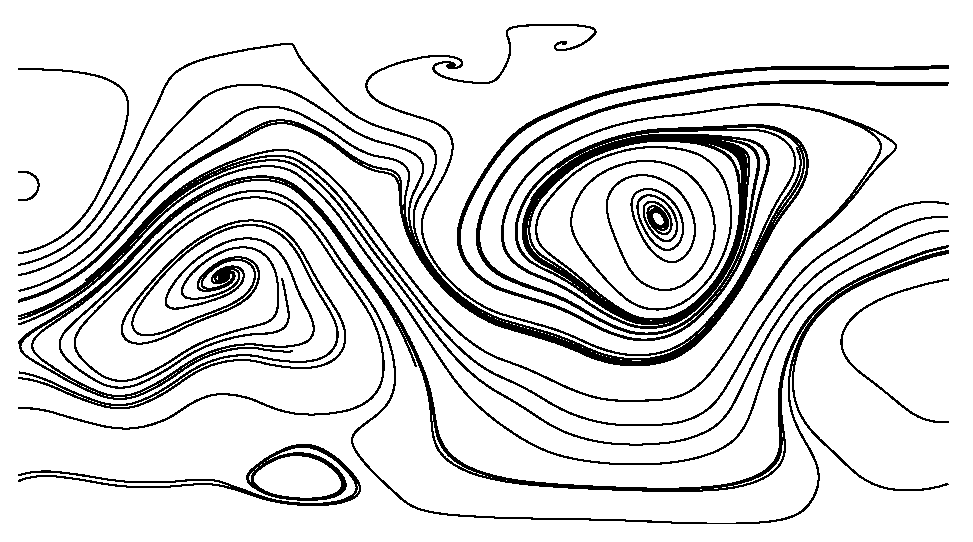
\includegraphics[height=3in]{streams.eps}
%\end{centering}
%\pagebreak
\tableofcontents
\thispagestyle{empty}
\pagebreak
\indent

%\begin{abstract}
%\end{abstract}

\pagestyle{plain}

\section{Introduction}

\begin{figure}
%\vspace{3.0in}
%\usepackage[dvips]{graphics}
\centering
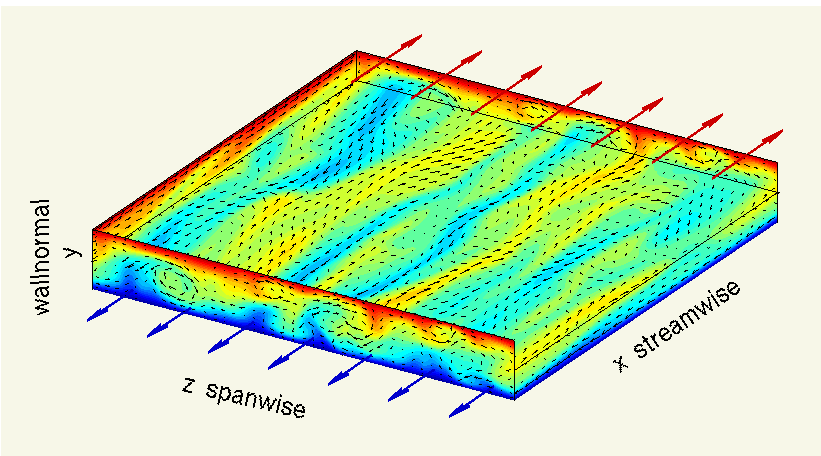
\includegraphics[width=0.8\textwidth]{ubigbox100}
\caption{{\bf Plane Couette flow simulated with Channelflow.} The flow is
driven by the motion of the upper and lower walls at $y = \pm 1$,
which travel with equal speeds in the $\pm x$-directions. Arrows
indicate in-plane velocities; the colormap indicates the speed of the
fluid in the $x$ direction: red/blue is $u = \pm 1$. The top half of
the fluid is cut away to show the flow at the $y=0$ midplane. The flow
domain is $[L_x, L_y, L_z] = [15,2,15]$ with periodic boundary
conditions in $x$ and $z$. The Reynolds number is 400, based on
channel half-height and half the relative wall velocity. The flow was
integrated on a $96 \times 33 \times 128$ grid with a fourth-order
backwards differentiation timestepping and a timestep of $dt = 0.02$.
Animations of this and other flows are available at
{\tt http://cns.physics.gatech.edu/}$\sim${\tt gibson/PCF-movies}.
}
\label{fig:couette}
\end{figure}




Channelflow is a direct numerical simulator for incompressible fluid
flow on a periodic, rectangular, wall-bounded domain. Channelflow uses
spectral discretization in spatial directions (Fourier x Chebyshev x
Fourier), finite-differencing in time, and primitive variables (3d
velocity and pressure) to integrate the incompressible Navier-Stokes
equations. The mathematics are based on the spectral channel-flow
algorithm in Section 7.3 of {\em Spectral Methods in Fluid Dynamics}
by Canuto, Hussaini, Quarteroni, and Zang (\cite{Canuto88}).
Channelflow is written in C++ and designed to be easy to use, easy to
understand, modular, extensible, and fast. Channelflow is documented,
licensed under the GNU GPL version 2, and available for download at

\begin{center}
\url{http://www.channelflow.org/download}
\end{center}

% points to make
% written in C++ for
% object-oriented programming techniques
%   abstraction,
%   data hiding
% type-checking
% memory management
%
% meant to work as a high-level programming language for spectral
% channelflow. falls short of that, due to C++ idiosyncracies, but
% close enough to
\subsection{Design}

Channelflow is written as a set of C++ classes that represent the
major components of spectral channel-flow simulation. The Channelflow
class library provides a high-level representation for expressing and
performing spectral channel-flow simulations. In Channelflow's
high-level syntax, fluids simulation programs are short, readable, and
easily modifiable. Channelflow falls short of a providing a {\em
language} for spectral simulation, due to the scope of the problem
domain and to the difficulty of presenting a clean syntax through C++
class libraries. But Channelflow should be good enough for a general
use by fluids researchers who need a fast, simple, and extensible way
to simulate channel flows.

Channelflow's classes are designed to be modular. Instances of classes
behave as independent objects with automatic memory management.
Auxiliary fields and computations can be added to a program with a few
lines of code. In Channelflow, even the DNS algorithm is an object.
This greatly increases the flexibility of DNS computations. For
example, a DNS object can be reparameterized and restarted multiple times
within a single program, multiple independent DNS computations can run
side-by-side within the same program, and DNS computations can run as
small components within a larger, more complex computations. As a
result, comparative calculations that formerly required coordination
of several programs through shell scripts and saved data files can
be done within single Channelflow program. In this way Channelflow
opens the way to a new class of computations that were not practically
possible with previous codes.

Channelflow uses object-oriented programming and data abstraction to
maximize the organization and readability of its library code, as
well. Channelflow defines about a dozen C++ classes that act as
abstract data types for the major components of spectral channel-flow
simulation, as outlined by CHQZ. Each class forms a level of
abstraction in which a set of mathematical operations are performed in
terms of lower-level abstractions, from time-stepping equations at the
top to linear algebra at the bottom. The Channelflow library code thus
naturally reflects mathematical algorithm, both in overall structure
and line-by-line. One can look at any part of the code and quickly
understand what role it plays in the overall algorithm. One can learn
the algorithm in stages, either top-down or bottom-up, by focusing
on one level of abstraction at a time.

Thus Channelflow has three main benefits:
\begin{itemize}
\item {\bf Ease of use:} Channelflow's high-level syntax allows
simple, rapid development of particular channel-flow simulations.
\item {\bf Modularity:} Its modularity allows a broader range of
channel-flow computations.
\item {\bf Intelligibility:} Its library code is organized and
documented in a way that makes learning the details easy.
\end{itemize}
Additional benefits are
\begin{itemize}
\item {\bf Extensibility:} Channelflow is adaptable to new needs. For
example, it is fairly easy to add a new time-stepping algorithm or
method of calculating the nonlinear term. It would not be difficult to
implement an
\item {\bf Speed:} Channelflow is as fast as comparable Fortran codes
\item {\bf Verifiability:} Channelflow contains a test suite
that verifies the correct behavior of major classes.
\item {\bf Documentation:} The documentation describes how to use
the software and precisely specifies the mathematics of the algorithm.
\end{itemize}


%In particular, I wrote channelflow because I found existing Fortran
%codes difficult to understand and use. The Fortran codes I examined
%were lean, mean, number-crunching machines. But as someone who grew up
%on structured and objected-oriented programming, I found it difficult
%to relate the Fortran codes' long sequence of low-level operations to
%the mathematical expressions in CQHZ's presentation of the algorithm.
%%I also anticipated that flat code structure and use of global
%variables would make moderate modifications difficult and, for
%%coordination of DNS results with other calculations of equal or
%greater complexity, would require independent programs, data exchange
%via files, and shell scripts to manage the coordination. I wanted to
%%avoid these things and learn the algorithm in detail, so I wrote
%channelflow.

%\subsection{Motivation}

%Why write a new channel-flow code when there are widely-used,
%well-tested, and efficient Fortran-77 codes?\footnote{all deriving
%from John Kim and Parviz Moin's work (\cite{Moin80}, \cite{Moin82})} I
%wrote channelflow primarily because I found existing Fortran codes
%difficult to understand and use.
%I cast no aspersions on these codes
%--they're lean, mean exemplars of F77 programming style. But as
%someone who grew up on structured and objected-oriented programming, I
%found it difficult to relate the Fortran codes' long sequence of
%low-level operations to the mathematical expressions in CQHZ's
%presentation of the algorithm. I also anticipated that flat
%code structure and use of global variables would make moderate
%modifications difficult and, for coordination of DNS results with
%other calculations of equal or greater complexity, would require
%independent programs, data exchange via files, and shell scripts to
%manage the coordination.
%%And as personal goals, I wanted to learn the
%%algorithm in depth, to get involved in free/open software development,
%%and to try my hand at bringing free/open software engineering
%%practices to the fluids research community (see Section
%\ref{software}).


\subsection{Drawbacks and rough edges}

The main potential drawbacks to using Channelflow have to do with C++.
C++ is a complex language that takes some getting used to. There will
be some learning overhead for those who are not familiar with it. How
much overhead depends on how deeply one wants to delve. Only very
basic knowledge of C++ is necessary for reparameterizing or modifying
the example programs. Modification of library code will require a fair
amount of experience. Secondly, C++ compilers vary in their
implementation of the language. Channelflow avoids the most complex
aspects of the C++ language to minimize portability problems and
learning overhead, but one can probably expect a few problems
compilation errors on new platforms. Channelflow was developed on
GNU/Linux with gcc-3.2. Dietmar Rempfer ported earlier versions of
Channelflow to MS-Windows and Visual C++, and the source code includes
his modifications as {\tt \#ifdefs}. Increasing Channelflow's
portability is a major goal for future releases.

%Perhaps the greatest downside of C++ is its inadequacy as a mechanism
%for language definition. Ideally, channelflow would have a clean, intuitive
%syntax
%I considered other languages before starting the difficulty of
%presenting a clean high-level syntax through class libraries. But it's
%better than other available

The following were not pressing concerns during the initial
development of Channelflow, but are getting more attention in
preparation for public release.
\begin{itemize}
\item {\bf Memory footprint:} Channelflow is memory-efficient with
large objects, such as flow fields that scale as $N^3$, but it is less
careful with small things, like making extra copies of parameters in
order to eliminate global variables. The wasted memory turns out to be
negligible. See Section \ref{sec:memory_benchmarks} for the details.
\item {\bf Import/export methods:} Most Channelflow modules have ASCII
or binary input and output methods. Some ASCII output is designed to
be readable by Matlab. Matlab scripts are provided for reading this
data into Matlab. There are not yet import/export methods for the
file formats of other channel-flow codes or for tools like Fluent and
Tecplot. It should be very easy to write these, if you know the format.
%See Section
\item {\bf Consistent nomenclature and syntax:} A number of inconsistencies
in this regard have become apparent during preparation of the documentation.
For example, {\tt Real unorm = L2Norm(u)} computes the $L^2$-norm of FlowField
{\tt u}, but {\tt Real udiv = u.divergence()} computes divergence. Some class
names could be changed.
\item {\bf Coverage of problem domain:} Channelflow aims to provide
elemental differential and algebraic operations for all its objects in
order to allow easy computation of arbitrary quantities. But so far
these operations have been written and tested on an as-needed basis,
so they are probably incomplete.
\item {\bf Graphical user interface:}  A basic GUI for setting parameters,
driving simulations, and plotting results would be quite useful.
\item {\bf Packaging:} At this point it might be necessary to edit the
Makefile to get Channelflow to compile. Ideally, Channelflow should
have an autoconf system (./configure; make) and be distributed in
RPM and Debian apt packages.
\end{itemize}
Help with any of these issues would be greatly appreciated.

\pagebreak

\section{Quick start}

Channelflow's C++ classes are compiled into software libraries. Under
normal circumstances, users of Channelflow should not need to modify
the Channelflow library code. Channelflow programs, on the other hand,
are relatively short sequences of statements that use the library
classes in particular ways to solve particular problems. The
Channelflow distribution includes several example programs that show
how this is done. Two of these are presented as annotated examples in
Section \ref{sec:examples}. Refer to the {\tt examples} directory for
other examples.

Most common simulation needs, such as the extraction of data or
statistics from the integration of an autonomous flow, can probably be
satisfied by modifications of the example programs. Complex problems
and unusual needs will call for novel arrangements of the classes and
possibly modification to the libraries.
%Section \ref{FOO}
%discusses extensions to the libraries. An example of fairly complex
%extensions to Channelflow is briefly described in \Sec{FOO}.

\subsection{Compilation}

On a Unix system, the following commands unpack the source distribution
and compile the libraries and a simple example program:
\begin{alltt}
  birbal\$ tar xvpfz channelflow-0.9.17.tgz
  birbal\$ cd channelflow-0.9.17/src
  birbal\$ make libs
  birbal\$ cd ../examples/couette
  birbal\$ make couette.x
  birbal\$ ./couette.x
\end{alltt}
To change the flow and integration parameters, edit {\tt couette.cpp}
and recompile. The other subdirectories of {\tt channelflow-0.9.17/examples}
have example programs for channel flow, Poisseuille flow, Orr-Sommerfeld
eigenfunctions, and the decay of a sinusoidal perturbation.

%For example, a plane
%Couette simulation differs from a channel flow simulation mostly by
%the definition of the base flow. For another example, two different
%integration techniques can be compared by constructing them, integrating
%them, and comparing their results within the same main program.

\subsection{Example programs}
\label{sec:examples}

This section presents several annotated Channelflow programs. The
programs are listed and the text steps explains what's happening,
line-by-line. The example programs are included in the Channelflow
distribution package in the {\tt examples} directory. See
\Sec{sec:installation} for information on compilation and execution.

Before launching into the examples, a few brief statements about the
the most important Channelflow classes: The {\bf FlowField} class
represents Fourier $\times$ Chebyshev $\times$ Fourier expansions of
vector fields on three-dimensional periodic domains. The {\bf DNS} class
represents a complete Navier-Stokes approximation method, that is, a
spatial discretization, a time-stepping algorithm, their parameters,
and the subsidiary data structures necessary to solve the discrete
equations. {\bf ChebyCoeff, ComplexChebyCoeff, BasisFunc} represent
Chebyshev expansions of real, complex, and vector-valued functions on
one-dimensional finite domains.


\subsubsection{couette.cpp: a simple program for plane Couette flow}
\label{sec:couette}

Code listing \ref{code:couette} shows the main body of a simple
Channelflow program, couette.cpp. The program integrates a plane
Couette flow with a linear base velocity profile, using 3rd-order
Runge-Kutta timestepping, constant pressure gradient, and a fixed time
step. The initial fluctuating velocity field consists of small
perturbations in the first few Fourier modes. The complete program is
included in the Channelflow distribution package in the {\tt
examples/couette} directory.

\begin{Code listing}
\small
\begin{alltt}
 {\it 1}  {\it (skip inclusion of header files)}
 {\it 2}
 {\it 3}  int main() \{
 {\it 4}
 {\it 5}    // Definition of numerical parameters Nx,Ny, etc.
 {\it 6}    {\it (skipped to save space)}
 {\it 7}
 {\it 8}    // Construct base flow for plane Couette: U(y) = y
 {\it 9}    ChebyCoeff U(Ny,a,b,Physical);
{\it 10}    Vector y = chebypoints(Ny, a,b);
{\it 11}    for (int ny=0; ny<Ny; ++ny)
{\it 12}      U[ny] = y[ny];
{\it 13}    U.save("U");
{\it 14}    y.save("y");
{\it 15}
{\it 16}    // Construct data fields: 3d velocity and 1d pressure
{\it 17}    FlowField u(Nx,Ny,Nz,3,Lx,Lz,a,b);
{\it 18}    FlowField q(Nx,Ny,Nz,1,Lx,Lz,a,b);
{\it 19}
{\it 20}    // Perturb velocity field
{\it 21}    u.addPerturbations(kxmax,kzmax,magnitude,decay);
{\it 22}
{\it 23}    // Construct a DNS object
{\it 24}    DNSFlags flags;
{\it 25}    flags.timestepping = RK3;  // use 3rd order Runge-Kutta method
{\it 26}    flags.constraint = BulkVelocity; // enforce bulk velocity
{\it 27}
{\it 28}    DNS dns(u, U, nu, dt, flags);
{\it 29}
{\it 30}    // Timestepping loop
{\it 31}    for (Real t=0.0; t<T; t += n*dt) \{
{\it 32}      cout << "============================================" << endl;
{\it 33}      cout << "         t == " << t << endl;
{\it 34}      cout << "       CFL == " << dns.CFL() << endl;
{\it 35}      cout << "L2Norm2(u) == " << L2Norm2(u) << endl;
{\it 36}
{\it 37}      // Save the kx=1,kz=2 Fourier profile
{\it 38}      ComplexChebyCoeff uprofile12 = u.profile(1,2,0);
{\it 39}      uprofile12.makePhysical();
{\it 40}      uprofile12.save("uprofile12"+i2s(int(t)));
{\it 41}
{\it 42}      // Take n steps of length dt
{\it 43}      dns.advance(u, q, n);
{\it 44}    \}
{\it 45}    u.binarySave("u");
{\it 46}    q.binarySave("q");
{\it 47}  \}
\end{alltt}
\normalsize
\caption{couette.cpp: a simple Channelflow program (line numbers added)}
\label{code:couette}
\end{Code listing}

\begin{supertabular}{p{1cm}p{12cm}}
line & meaning \\\hline
1--7 & The code listing skips the header-file
inclusion statements and parameter definitions to save space. The
parameter definitions take the form {\tt int Nx=32; Real Lx = 2*pi;}
etc.
\\
8--14 & The base flow {\tt U} is declared as a variable of type
ChebyCoeff and the $y$-gridpoints {\tt y} are set as a real-valued
Vector. The for-loop sets the base flow to a linear profile, $U(y) = y$.
Both {\tt U} and {\tt y} are set and saved to disk in an ASCII
Matlab-readable format.
\\
17--18 & The fluctuating velocity {\tt u} and modified pressure {\tt q}
fields are allocated and initialized to zero. The FlowField
constructor allocates memory for 3d and 1d $N_x \times N_y \times N_z$
grids, respectively. The domain of each field is set to $[0,L_x] \times [a,b]
\times [0,L_z]$.
\\
21 & Random divergence-free perturbations are added to Fourier
modes with {\tt |kx| < kxmax} and {\tt |kz| < kxmax}. The {\tt magnitude}
and {\tt decay} parameters determine the spectral characteristics of
the perturbations' Chebyshev expansions along $y$.
\\
24--26 & The next few statements construct a DNSFlags object and modify
a few of its default values.
\\
28 & The DNS constructor allocates and initializes data needed for
time-stepping calculations, based on the initial velocity field, the
base flow, the viscosity, the timestep, and the flags.
\\
31--35 & A for-loop advances time from {\tt T0} to {\tt T1}
in steps of length {\tt n*dt}. At each step, the time the CFL number,
and the $L_2$-norm of the velocity field are printed out.
\\
38--40 & The Fourier profile $\tu_{12}(y)$ is extracted from
velocity field {\tt u}, transformed from spectral representation to
physical gridpoint values, and then saved to disk in ASCII Matlab-readable
form, with filenames indicating the integration time.
\\
43 & The DNS object {\tt dns} advances the velocity and pressure fields
{\tt n} steps of length {\tt dt}.
\\
45--46 &  After the time-stepping loop finishes, the
velocity and modified pressure fields are saved to disk in binary
form and the main program.
\\
\end{supertabular}

\vspace{0.1in}
Of course, what's notable about couette.cpp is what {\em doesn't}
appear, for example, allocation of arrays, Fourier transforms,
calculation of nonlinear terms, influence-matrix calculations, and
solution of linear algebra problems. These operations are carried out
internally by the objects to which they pertain. Most of the work
occurs within DNS construction (line 28, {\tt DNS(u,U,nu,dt,flags))},
and the DNS advance function (line 43, {\tt dns.advance(u,q,n)}).

\subsubsection{couette2.cpp: variable time-stepping, statistics, and start-up
from saved fields}
\label{sec:couette2}

The couette2.cpp example program adds to couette.cpp variable time-stepping,
simple statistics, and start-up from saved field to couette.cpp. The
statistics calculated in couette2.cpp are the mean-velocity profile and the
mean drag on the lower wall. Code listings \ref{code:couette2a} and
\ref{code:couette2b} show the program in its entirety. The program is
included in the Channelflow source distribution at
{\tt examples/couette/couette2.cpp}.


\begin{Code listing}
\begin{alltt}
\small
{\it  1}  #include <iostream>
{\it  2}  #include <iomanip>
{\it  3}  #include "vector.h"
{\it  4}  #include "chebyshev.h"
{\it  5}  #include "flowfield.h"
{\it  6}  #include "nsintegrator.h"
{\it  7}
{\it  8}  int main() \{
{\it  9}
{\it 10}    // Define flow parameters
{\it 11}    const Real Reynolds = 400.0;
{\it 12}    const Real nu = 1.0/Reynolds;
{\it 13}
{\it 14}    // Define integration parameters
{\it 15}    const Real dtmax = 0.15;
{\it 16}    const Real dtmin = 0.05;
{\it 17}    const Real CFLmax = 0.90;
{\it 18}    const Real CFLmin = 0.5;
{\it 19}    const Real dT  = 1.0;     // plot interval
{\it 20}    const Real T0  = 100.0;    // start time
{\it 21}    const Real T1  = 200.0;    // end time
{\it 22}
{\it 23}    // Load velocity, modified pressure, and base flow from disk.
{\it 24}    FlowField u("u100");
{\it 25}    FlowField q("q100");
{\it 26}    ChebyCoeff U("U");
{\it 27}
{\it 28}    // Get y-domain information from velocity field.
{\it 29}    Real a = u.a();
{\it 30}    Real b = u.b();
{\it 31}    int Ny = u.Ny();
{\it 32}
{\it 33}    // Construct a DNS object
{\it 34}    DNSFlags flags;
{\it 35}    flags.timestepping = RK3;
{\it 36}    flags.constraint = PressureGradient;
{\it 37}
{\it 38}    TimeStep dt((dtmax+dtmin)/2, dtmin, dtmax, dT, CFLmin, CFLmax);
{\it 39}    DNS dns(u, U, nu, dt, flags, T0);
{\it 40}
{\it 41}    ChebyCoeff u00mean(Ny,a,b,Spectral);
{\it 42}    Real dragmean = 0.0;
{\it 43}    int count = 0;
\end{alltt}
\normalsize
\caption{couette2.cpp: variable time-stepping, statistics,
and start-up from saved fields}
\label{code:couette2a}
\end{Code listing}

\begin{Code listing}
\begin{alltt}
\small
{\it 44}
{\it 45}    for (Real t=T0; t<T1; t += dT) \{
{\it 46}
{\it 47}      // Get kx=kz=0 Fourier component u00(y) and compute drag
{\it 48}      ChebyCoeff u00 = Re(u.profile(0,0,0));
{\it 49}      ChebyCoeff du00dy = diff(u00);
{\it 50}      Real drag = nu*du00dy.eval_a();
{\it 51}
{\it 52}      u00mean += u00;
{\it 53}      dragmean += drag;
{\it 54}      ++count;
{\it 55}
{\it 56}      // Save stuff
{\it 57}      string time = i2s(int(t));
{\it 58}      u00.save("uprofile00_"+time);
{\it 59}      Re(u.profile(1,2,0)).save("uprofile12_"+time);
{\it 60}
{\it 61}      cout << "==========================================" << endl;
{\it 62}      cout << "         t == " << t << endl;
{\it 63}      cout << "        dt == " << dt << endl;
{\it 64}      cout << "       CFL == " << dns.CFL() << endl;
{\it 65}      cout << "L2Norm2(u) == " << L2Norm2(u) << endl;
{\it 66}      cout << "      drag == " << drag << endl;
{\it 67}
{\it 68}      // Take n steps of length dt
{\it 69}      dns.advance(u, q, dt.n());
{\it 70}
{\it 71}      // Adjust timestep if CFL number is too large or too small.
{\it 72}      if (dt.adjust(dns.CFL())) \{
{\it 73}        cout << "adjusting timestep" << endl;
{\it 74}        dns.reset(nu, dt);
{\it 75}      \}
{\it 76}    \}
{\it 77}
{\it 78}    // Compute means
{\it 79}    dragmean /= count;
{\it 80}    u00mean /= count;
{\it 81}
{\it 82}    // Fourier-transform u00mean, save, and print
{\it 83}    u00mean.makePhysical();
{\it 84}    u00mean.save("u00mean");
{\it 85}    cout << "mean drag == " << dragmean << endl;
{\it 86} \}
\end{alltt}
\normalsize
\caption{couette2.cpp cont'd: variable time-stepping, statistics,
and start-up from saved fields}
\label{code:couette2b}
\end{Code listing}

\begin{tabular}{p{2cm}p{12cm}}
line & meaning \\\hline
1-6 & These header-file inclusion statements declare standard
C++ I/O classes and a number of Channelflow classes.
\\
11-21 & Definitions of flow and integration parameters.
\\
24-26 & Load the velocity, the modified pressure, and
the base flow that were saved to disk in {\tt couette.cpp}. Channelflow's
binary storage format for FlowFields includes data such as the gridsize,
the domain, and the Physical/Spectral state of the data, in addition to
the data itself. Thus the FlowField {\tt u} at line 24 is reconstructed
in exactly the same state as the FlowField saved at at line 45 in
{\tt couette.cpp}. {\tt ChebyCoeff} uses an ASCII, Matlab-readable
file format, with parametric information stored in a comment line.
\\
29-31 & Extract information about the $y$-domain from FlowField
{\tt u}.
\\
34-36 & Set a few flags for the DNS.
\\
 38 & Construct a TimeStep object for variable time-stepping.
The initial timestep is set halfway between its minimum and maximum bounds.
The timestep {\tt dt} will vary during the integration to keep the CFL
number and the timestep between the given bounds, but always as a
whole-number fraction of the plot  interval {\tt dT}, i.e. $dt = dT/n$
for some integer $n$.
\\
 39 & Construct a DNS based on the velocity field {\tt u}, the base flow
{\tt U}, viscosity {\tt nu}, TimeStep {\tt dt}, and starting time {\tt T0}.
The starting time of {\tt couette2.cpp} equals the end time of
{\tt couette.cpp}.
\\
41-43 & Construct variables for accumulating sums for the
calculation of the mean drag and the mean $k_x,k_z=0,0$ Fourier profile.
\\
 45 & Begin time-stepping loop. Note that time increases by
the plot interval {\tt dT} each pass through the loop.
\\
48-50 & Extract Fourier profile $\tu_{00}(y)$, compute
$\Re(\del \tu_{00} / \del y)$, and $\nu \Re(\del \tu_{00} / \del y |_{y=a})$.
Line 50 uses a special efficient function for evaluating ChebyCoeffs at
an endpoint.
\\
52-54 & The current values of $\tu_{00}(y)$ and the drag
are added into their summation variables.
\\
57-59 & Save the current $\tu_{00}(y)$ and $\tu_{12}(y)$
profiles to disk, with file names that indicate the integration time.
Line 59 illustrates how to save a profile to disk without the use of
a temporary ChebyCoeff variable.
\\
61-66 & Print interesting information.
\\
 69 & Advance {\tt n} timesteps of length {\tt dt}.
\\
72-74 & Check if the CFL condition is out of bounds and
adjust if necessary. If adjustment occurs, the {\tt dt.adjust}
function returns {\tt true}, and the DNS object {\tt dns} is
recalibrated for the new timestepping interval.
\\
79-80 & Divide the sums by the number of samples to get the means.
\\
83-85 & Transform {\tt u00mean} to gridpoint values, save to disk,
 and print the mean drag.
\end{tabular}


\section{Guide to main classes}
\label{sec:chebyshev}

This section is a user's guide to the behavior and meaning of the main
Channelflow classes. The goal is to discuss how to use and control the
main classes in top-level Channelflow programs. Parts of the DNS
class are in full mathematical detail in \Sec{sec:math_details}. At this
point the documentation falls short of an exhaustive reference manual.
Please consult the header files and source code for more information.

\subsection{ChebyCoeff}
\label{sec:chebycoeff}

\subsubsection{Description}

The ChebyCoeff class represents real-valued Chebyshev expansions
of functions on the domain $[a,b]$, of the form
\begin{align}
f(y) = \sum_{n=0}^{N-1} \widehat{f}_n \bar{T}_n(y)
\label{eqn:chebyexpan}
\end{align}
where $\bar{T}_n(y)$ is the $n$th Chebyshev polynomial rescaled to the
interval $y \in [a,b]$. That is,
\begin{align}
\bar{T}_n(y) = T_n\left(\frac{2y-(b+a)}{b-a}\right)
\end{align}
ChebyCoeffs are on a general domain $[a,b]$ instead of the usual $[-1,
1]$ to facilitate programs that involve more than one approximation
domain. In general the right-hand side of \eqn{eqn:chebyexpan} is an
approximation of a function $f$. For simplicity, we treat the function
and its expansion as identically equal.

The spectral coefficients of a function $f$ can be computed
efficiently from the function values taken at a discrete set of
Chebyshev gridpoints. Let
\begin{align}
y_n &= \frac{b+a}{2} + \frac{b-a}{2} \cos\left(\frac{n \pi}{N-1}\right),
\:\:\:\: n \in [0, N-1]
\end{align}
and let $f_n = f(y_n)$. Then a fast cosine transform can be used to
transform the function values $\{f_0, f_1, \ldots, f_{N-1}\}$ into the
spectral coefficients $\{\hf_0, \hf_1, \ldots, \hf_{N-1}\}$, and vice
versa. The main point of the ChebyCoeff class is to store an array of
these function values or Chebyshev spectral coefficients, transform
back and forth between them, and approximate properties of the function
$f(y)$ based on the spectral expansion \ref{eqn:chebyexpan}.

\subsubsection{Data access, transforms, and state}

The ChebyCoeff class has a data array that stores either function
values or spectral coefficients and a flag that indicates which state
the data array is in. For the ChebyCoeff object {\tt f}, elements of
the data array are accessed with the square-bracket operator, e.g.
{\tt f[n]}. The function {\tt f.state()} returns {\tt Physical} if the
array represents function values and {\tt Spectral} if spectral
coefficients. The Physical/Spectral state is set at construction time
and toggled when the ChebyCoeff's transform functions are called. For
example, the following block of code constructs a length-$N$
ChebyCoeff object {\tt f} on the domain $[-1,1]$, sets the function
values $\{f_n\}$ to $\{\sin(\pi y_n)\}$, transforms the ChebyCoeff from
{\tt Physical} to {\tt Spectral}, and then prints the zeroth spectral
coefficient.
\begin{alltt}
  Vector y = chebypoints(N,-1,1);
  ChebyCoeff f(N,-1,1,Physical);

  for (int n=0; n<N; ++n)
    f[n] = sin(pi*y[n]);

  if (f.state() == Physical)  // will be true
    f.chebyfft();             // transform f from Physical to Spectral
  cout << f[0] << endl;       // print coeff of T_0

  if (f.state() == Spectral)  // will be true
    f.ichebyfft();            // transform f from Spectral to Physical
  cout << f[0] << endl;       // print value of sin(pi*y[0])
\end{alltt}
Note that the return-value of {\tt f.state()} is a variable of type {\tt
fieldstate}, with two possible values: {\tt Physical} and {\tt
Spectral}.

Several other forms of transform function are provided for convenience
and efficiency. The functions
\begin{alltt}
    f.makeSpectral();  // if f.state()!=Spectral, transform to Spectral
    f.makePhysical();  // if f.state()!=Physical, transform to Physical
\end{alltt}
are state-checking versions of {\tt f.chebyfft()} and {\tt f.ichebyfft()}.
Using these forms eliminates the possibility of performing the same
transform twice in a row. A third form performs the transform specified
by an argument. If {\tt s} be a variable of type {\tt fieldstate}, then
\begin{alltt}
    f.makeState(s);  // if f.state()!=s, transform to state s
\end{alltt}
transforms {\tt f} to that state {\tt s}.

Each of the transforms discussed so far has a more efficient form
that takes a {\tt ChebyTransform} argument. The {\tt ChebyTransform}
class is described in \Sec{sec:chebytransform}. For now, suffice it to
say that some common work can be factored out of multiple calls to
{\tt ChebyCoeff} transforms of equal length by constructing a
{\tt ChebyTransform} object and passing it to the {\tt ChebyCoeff}
transform functions, as in
\begin{alltt}
    int N = f.length();
    ChebyTransform trans(N);

    f.chebyfft(trans);
    f.ichebyfft(trans);
    f.makeSpectral(trans);
    f.makePhysical(trans);
    f.makestate(trans, s);
\end{alltt}
These forms are the preferred forms for {\tt ChebyCoeff} transforms.
They should be used in frequently repeated calculations. The forms without
{\tt ChebyTransform} arguments are conveniences for use when efficiency
is not an issue.

For a more complete discussion of the numerics of Chebyshev approximation,
cosine transforms, and the FFT, see {\em Numerical Recipes in C}
(\cite{Press88}). But don't implement Numerical Recipe's algorithm! It's
less numerically stable than FFTW's algorithm (termed RDEFT, for
``Discrete Real Even Fourier Transform'').

\subsubsection{Input/output}

{\tt ChebyCoeff} I/O is done with a {\tt save} function and a constructor
that both take a filename argument. For example, given a {\tt ChebyCoeff f},
\begin{alltt}
  string filebase = "foo";
  f.save(foo);

  ChebyCoeff g(filebase);
\end{alltt}
saves {\tt f} to disk in file {\tt foo.asc} and then constructs {\tt g}
based on the data stored in the file. At after construction, {\tt g}
will be identical to {\tt f}, with the same length, bounds, state, and
data.

The ASCII file format for {\tt ChebyCoeff} is
\begin{alltt}
\%{\em N a b s
f[0]
f[1]
.
.
.
f[N-1]}
\end{alltt}
where $N$ is the integer expansion length, $a$ and $b$ are the
double-precision domain bounds, $s$ is a character {\tt P} or {\tt S},
indicating the {\tt Physical} or {\tt Spectral} state, and the $f[n]$
are double-precision values of function values or spectral coefficients.
The {\tt \%} character marks the first line as a comment in Matlab,
so that the file can be read into Matlab as an $N \times 1$ matrix
with the command {\tt load foo.asc}.

\subsubsection{Other functions}

{\tt ChebyCoeff} provides a number of other functions for arithmetical
operations, computing norms, derivatives, etc. Note that most of these
functions operate on spectral coefficients and so require the
{\tt ChebyCoeff} to be in {\tt Spectral} state. Please refer to the
header files for a complete list of functions. A few quick examples:
\begin{alltt}
  ChebyCoeff f(N,a,b,Spectral);
  ChebyCoeff g(N,a,b,Spectral);

  f.randomize(magn, decay); // set f[n] = magn*random()*pow(decay,n)
  g.randomize(magn, decay); // ditto for g

  f += g;                   // add g to f;
  Real x = L2Dist2(f,g);    // 1/(b-a) Integral_a^b (f-g)^2 dy
  Real y = chebyNorm2(f);   // 2/(b-a) Integral_a^b f^2/sqrt((y-a)(b-y)) dy

  ChebyCoeff dfdy = diff(f);   // compute derivative of f
  ChebyCoeff F = integrate(f); // compute integral of f, set F.mean() to 0

  Real f_a = f.eval_a();       // return function value at lower bound
  Real f_m = f.eval((b+a)/2);  // return function value at midpoint
\end{alltt}


\subsection{ComplexChebyCoeff}
\label{sec:complexchebycoeff}

{\tt ComplexChebyCoeff} represents complex-valued Chebyshev expansions
of the form of \eqn{eqn:chebyexpan} and follows the same syntax as
{\tt ChebyCoeff} in almost all respects. There's just one thing to watch
out for: {\em you can't assign into } {\tt f[n]}! Or rather, you can
assign into {\tt f[n]}, and it will compile and run with no complaints,
but it won't have any effect on the value of {\tt f[n]}. To set the
value of {\tt f[n]}, use
\begin{alltt}
   f.set(n, z);  // CORRECT: sets f[n] to z
\end{alltt}
and not
\begin{alltt}
   f[n] = z;     // INCORRECT: doesn't change f[n]
\end{alltt}
This behavior is due to a bad design decision that I hope to correct
before the channelflow-1.0.0 release. The {\tt f[n]} syntax works just
fine for extracting spectral coefficients or function values.
\begin{alltt}
   Complex z = f[n];  // OK: sets z to f[n]
\end{alltt}


The {\tt ComplexChebyCoeff} I/O methods follow the same syntax as
{\tt ChebyCoeff}, but the ASCII file format has two columns for the real
and imaginary parts of the data
\begin{alltt}
\%{\em N a b s
Re(f[0]) Im(f[0])
Re(f[1]) Im(f[1])
.
.
.
Re(f[N-1]) Im(f[N-1)}
\end{alltt}

Other numerical functions are the usual complex generalizations.
For example, {\tt L2InnerProduct2(f,g)} computes $1/(b-a) \int_a^b f g^* dy$.


\subsection{ChebyTransform}
\label{sec:chebytransform}

{\tt ChebyTransform} is a wrapper class for the discrete cosine transforms
of the elegant and powerful FFTW3 library, by Matteo Frigo and
Steven G.\ Johnson (see \url{www.fftw.org} and \cite{Frigo98}). In order
to use {\tt ChebyTransform} well, one should know a few things about FFTW.
FFTW uses code generation and run-time profiling to find the optimal
FFT algorithm for given transform length on a given processor. Once
that optimal FFT is found, it can be reused as many times as needed.
Thus optimal use of FFTW consists of a relatively high-cost ``learning''
phase and repeated execution of the optimal FFT algorithm. If only a
single transform needs to be calculated, a good algorithm can be estimated
with heuristics or the results of previous learning. FFTW's accumulated
learning is called ``wisdom.'' Wisdom can be saved to disk and recalled
in subsequent runs.

The {\tt ChebyTransform} class does FFTW's learning or estimating during
construction and repeated execution in calls to its transform functions.
The {\tt ChebyTransform} constructor takes an integer {\tt N} argument
that specifies the transform length and an optional integer flag argument
that specifies how FFTW should learn or estimate. The default behavior
is wisdom-based estimation rather than learning. For example,
\begin{alltt}
  ChebyTransform trans(N);
\end{alltt}
constructs a {\tt ChebyTransform} with wisdom-based estimation of the
optimal FFT for length N.
\begin{alltt}
  ChebyTransform trans(N, FFTW_MEASURE);
\end{alltt}
performs the high-cost ``learning'' phase to find a nearly optimal
length-$N$ transform.
\begin{alltt}
  ChebyTransform trans(N, FFTW_MEASURE | FFTW_WISDOM);
\end{alltt}
learns the optimal transform and adds remembers it to improve any subsequent
estimates. The {\tt FFTW\_PATIENT} flags can be substituted in place of
{\tt FFTW\_MEASURE} to run a more exhaustive search and find a more nearly
optimal algorithm. For exact details on FFTW flags, see the FFTW documentation.
Channelflow provides two methods for saving FFTW wisdom to disk and
rereading it, {\tt fftw\_loadwisdom()} and {\tt fftw\_savewisdom()}, both
taking an optional filename argument. The filename defaults to
\url{~/.fft-wisdom} if left unspecified.

I generally load wisdom at the beginning of my programs and save it at
the end. However, I recommend reading the FFTW documentation on
wisdom. You can undermine the performance of Channelflow by developing
wisdom on one machine architecture and using it on another.

\subsection{FlowField}
\label{sec:flowfield}

% order of discussion
% pragmatic
%   transforms
%   state-checking
%   data access
%   layout
%   bounds

% mathematical
%   definitions of transforms
%   calculation by FFTW

The FlowField class represents vector-valued Fourier $\times$ Chebyshev
$\times$ Fourier expansions whose mathematical form is
\begin{align}
\bu(\bx) &= \sum_{k_x=-N_x/2+1}^{N_x/2} \; \sum_{n_y=0}^{N_y-1} \; \sum_{k_z=-N_z/2+1}^{N_z/2}
\htbu_{k_x,n_y,k_z} \bar{T}_{n_y}(y) \; e^{2 \pi i \left(k_x x/L_x + k_z z/L_z \right)}
\label{eqn:flowfield_expansion_math}
\end{align}
where $N_x$ and $N_z$ are even, $\bx = (x,y,z)$, and $\bar{T}_m$ is
the $m$th Chebyshev polynomial rescaled for the domain $y \in [a,b]$.
For $N_x$ odd, the sum is over $k_x = -N_x/2+1$ to $N_x/2-1$, and
likewise for $N_z$. The double tilde/hat notation on the spectral
coefficients indicates that the coefficients result from a combined
Fourier transform in $xz$ and a Chebyshev transform in $y$.

The primary function of FlowField, like ChebyCoeff, is to store data
in arrays, transform it back and forth from Spectral and Physical
representations, allow access to the physical data or spectral
coefficients, and perform mathemtical operations related to the
spectral expansions. FlowField, however, is considerably more
complicated, so we discuss it in greater detail.

%The transforms, states, and data access methods are more complicated
%than those of ChebyCoeffs because (1) the $xz$ and $y$ transforms are
%independent, (2) $xz$ transforms switch the data between Real and
%Complex types, and (3) the storage of the Complex data takes advantage
%of symmetries obeyed by the transforms of Real-valued data.

\subsubsection{A few examples of use}

The following code snippet declares a 3d FlowField on $(N_x, N_y, N_z)$
gridpoints, on the box $[0, L_x] \cross [a, b] \cross [0, L_z]$, sets
the field to physical values provided by an external function, and then
transforms the field to a spectral representation

\begin{alltt}
  FlowField u(Nx,Ny,Nz,3,Lx,Lz,a,b,Physical,Physical);

  Vector x = u.xgridpts();
  Vector y = u.ygridpts();
  Vector z = u.zgridpts();

  for (int i=0; i<3; ++i)
    for (int ny=0; ny<Ny; ++ny)
      for (int nx=0; nx<Nx; ++nx)
        for (int nz=0; nz<Nz; ++nz)
          u(nx,ny,nz,i) = f(x(nx), y(ny), z(nz), i);

  u.makeSpectral();
\end{alltt}

The next code snippet declares a 3d FlowField in the default
{\tt Spectral, Spectral} state, assigns successively smaller random
values to the Chebyshev coefficients of the $(k_x , k_z)
= (-1, 4)$ Fourier mode, computes the curl of the field, ouputs the
$L_2$ norm of the curl, and then transforms and prints the curl's
physical gridpoint values.

\begin{alltt}
  FlowField f(Nx,Ny,Nz,3,Lx,Lz,a,b);

  int kx = -1;
  int kz =  4;
  int mx = u.mx(kx);
  int mz = u.mz(kz);
  Real magn = 1.0;
  Real decay = 0.5;

  for (int my=0; my<f.My(); ++my) \{
    for (int i=0; i<f.Nd(); ++i)
      f.cmplx(mx,my,mz,i) = magn*randomComplex();
    magn *= decay;
  \}

  FlowField g = curl(f);
  cout << "L2Norm(curl u) == " << L2Norm(g) << endl;

  g.makePhysical();
  for (int i=0; i<g.Nd(); ++i)
    for (int nx=0; nx<g.Nx(); ++nx)
      for (int ny=0; ny<g.Ny(); ++ny)
        for (int nz=0; nz<g.Nz(); ++nz)
          cout << g(nx,ny,nz,i) << ' ';

\end{alltt}

\subsubsection{Mode numbers, wave numbers, and grid points}

Fun facts about FlowFields:
\begin{itemize}
\item FlowFields are allocated in terms of their physical grid sizes
$N_x \times N_y \times N_z$ and vector dimension $N_d$.
\item Physical gridpoint data is real-valued, indexed by
{\bf gridpoint indices} $(n_x, n_y, n_z)$, and accessed with syntax
{\tt u(nx,ny,nz,i)}.
\item Spectral coefficient data is complex-valued, indexed by
{\bf mode numbers} $(m_x, m_y, m_z)$, and accessed with syntax
{\tt u.cmplx(mx,my,mz,i)}.
\item However, FlowField's $xz$ and $y$ transforms are independent,
so that mixed Physcial,Spectral and Spectral,Physical states are
possible, too.
\item {\tt u.Nx()}, {\tt u.Ny()}, and {\tt u.Nz()} indicate the
{\bf number of gridpoints} in $x,y,$ and $z$ for a given FlowField.
\item {\tt u.Mx()}, {\tt u.My()}, and {\tt u.Mz()} indicate the
{\bf number of modes} in $x,y,$ and $z$ for a given FlowField.
\item The ranges of gridpoint indices are $0 \leq n_x < N_x$, etc.
\item The ranges of mode numbers are  $0 \leq m_x < M_x$, etc.
\item Because FlowField's Fourier transform maps Real-valued gridpoint
data into (roughly) half as many Complex-valued spectral coefficients,
the number of gridpoints differs from the number of modes. In particular,
\begin{align}
M_x &= N_x \\
M_y &= N_y \\
M_z &= N_z/2+1
\end{align}
\item The mode numbers $m_x$ and $m_z$ are merely indices into the
complex array of spectral coefficients; they are {\em not} equal
to the Fourier {\bf wave numbers} $k_x$ and $k_z$ that appear in
\eqn{eqn:flowfield_expansion_math}. However, the two are related by
\begin{align}
m_x &= \begin{cases}
	k_x+M_x & -M_x/2+1 \leq k_x < 0 \\
	k_x & 0 \leq k_x \leq M_x/2
        \end{cases} \\
m_z &= \begin{cases}
	k_z & 0 \leq k_z < M_z \\
        \text{undefined} & k_z < 0
        \end{cases}
\intertext{and}
k_x &= \begin{cases}
	m_x & 0 \leq m_x \leq M_x/2 \\
	m_x - M_x & M_x/2 < m_x < M_x
        \end{cases}\\
k_z &=  m_z \quad 0 \leq m_z < M_z
\end{align}
\item Gridpoint indices are related to the coordinates of gridpoints by
\begin{alignat}{2}
x_{n_x} &= \frac{n_x L_x}{N_x}  & 0 \leq n_x < N_x \label{eqn:xnx} \\
y_{n_y} &= \frac{b+a}{2} + \frac{b-a}{2} \cos\left(\frac{n_y \pi}{N_y-1}\right) & \quad 0 \leq n_y < N_y \label{eqn:yny} \\
z_{n_z} &= \frac{n_z L_z}{N_z}  & 0 \leq n_z < N_z \label{eqn:znz}
\end{alignat}

\end{itemize}

\subsubsection{FlowField states, access methods, and transforms}

The primary functions of FlowField are to store data, either as
spectral coefficients $\htbu_{m_x,m_y,m_z}$ or as physical gridpoint
values $\bu(x_{n_x},y_{n_y},z_{n_z})$, and to transform between
spectral and physical representations as needed. FlowField performs
its $x,z$ Fourier transforms together and its $y$ Chebyshev transform
separately, so that a FlowField can be in any one of four states:

\noindent Tildes ($\: \widetilde{u}\:$) denote Fourier coefficients; hats
($\:\widehat{u}\:)$ Chebyshev coefficients. In what follows we use the
abbreviations PP, PS, SP, and SS for the four states of FlowFields,
with the $xz$ state listed first.

FlowFields can be initialized in any of the four states. For example,
\begin{alltt}
  FlowField u(Nx,Ny,Nz,Lx,Lz,a,b,Physical,Spectral);
\end{alltt}
constructs a FlowField in state PS. FlowField has two functions for
checking state:
\begin{alltt}
  fieldstate xzstate = u.xzstate();
  fieldstate ystate  = u.ystate();
\end{alltt}
A {\tt fieldstate} has value {\tt Physical} or {\tt Spectral}.


\subsubsection{FlowField access methods}

As noted above, the $xz$ Fourier transform applied to a P* FlowField
puts the FlowField in S* state and switches its data from real-valued
to complex-valued. FlowField has separate functions for accessing
real and complex-valued data. For example, real-valued P* FlowField
data is set with
\begin{alltt}
   u(nx,ny,nz,i) = 4.0;               // for u in state P*
\end{alltt}
Complex-valued S* FlowField data is set with
\begin{alltt}
   u.cmplx(mx,my,mz,i) = 4.0 + 3.0*I; // for u in state S*
\end{alltt}
You {\em must} use the data access method that is appropriate for the
FlowField's $xz$ state. Using the wrong access method will corrupt
FlowField data and lead to meaningless results. To ensure correct use,
Channelflow provides debugging libraries that check FlowField state
during each data access call. If the access method doesn't match the
state, an error message will be printed and execution will stop. If
you're unsure of the correctness of your code, link to the debugging
libraries and run. See \Sec{sec:debugging}.

The meaning of the assignments in the above examples depends further
on the FlowField's {\tt ystate}. For example, the above complex
assignment sets the value of $\widetilde{u}_{i,m_x,m_z}(y_{m_y})$ if
{\tt u} is in state SP and $\widehat{\widetilde{u}}_{i,m_x,m_y,m_z}$
if {\tt u} is SS.

\begin{table}
\centering
\caption{{\bf FlowField states and access functions.} }
\label{tbl:ffstates}
\vspace{2mm}
\begin{tabular}{c|rlllc}
$xz,y$ state & access function & mathematical meaning & type & description  \\\hline
Physical, Physical & {\tt u(nx,ny,nz,i)} & $u_i(x_{n_x},y_{n_y},z_{n_z})$ & Real & gridpoint values\\
Physical, Spectral & {\tt u(nx,my,nz,i)} & $\widehat{u}_{i,m_y}(x_{n_x},z_{n_z})$ & Real & mixed state\\
Spectral, Physical & {\tt u.cmplx(mx,ny,mz,i)} & $\widetilde{u}_{i,m_x,m_z}(y_{n_y})$ & Complex & mixed state\\
Spectral, Spectral & {\tt u.cmplx(mx,my,mz,i)} & $\widehat{\widetilde{u}}_{i,m_x,m_y,m_z}$ & Complex & spectral coeffs
\end{tabular}
\end{table}

FlowField provides conversion functions for array indices, gridpoint
positions, and wavenumbers:
\begin{alltt}
  Real x = u.x(nx);   // get the x coordinate of the nxth gridpoint
  Real y = u.y(ny);
  Real z = u.z(nz);

  int kx = u.kx(mx);  // get the wavenumber kx of the mxth mode
  int kz = u.kz(mz);

  int mx = u.mx(kx);  // get the mode number mx of the kxth Fourier mode
  int mz = u.mz(kz);
\end{alltt}
Other functions provide bounds for the spatial indices. For example,
a PP FlowField can be set to zero by
\begin{alltt}
  for (int i=0; i<u.Nd(); ++i)
    for (int ny=0; ny<u.Ny(); ++ny)
      for (int nx=0; nx<u.Nx(); ++nx)
        for (int nz=0; nz<u.Nz(); ++nz)
           u(nx,ny,nz,i) = 0.0;
\end{alltt}
whereas an SS FlowField is can be zeroed with
\begin{alltt}
  Complex zero = 0.0 + 0.0*I;
  for (int i=0; i<u.Nd(); ++i)
    for (int my=0; my<u.My(); ++my)
      for (int mx=0; mx<u.Mx(); ++mx)
        for (int mz=0; mz<u.Mz(); ++mz)
           u.cmplx(mx,my,mz,i) = zero;
\end{alltt}

\subsubsection{FlowField transform functions}
\label{sec:FFtransforms}

The FlowField transform functions are
\begin{alltt}
  u.realfft_xz();         // P* -> S*
  u.irealfft_xz();        // S* -> P*
  u.chebyfft_y();         // *P -> *S
  u.ichebyfft_y();        // *S -> *P

  u.makeSpectral_xz();    // ** -> S*
  u.makePhysical_xz();    // ** -> P*
  u.makeSpectral_y();     // ** -> *S
  u.makePhysical_y();     // ** -> *P

  u.makeSpectral();       // ** -> SS
  u.makePhysical();       // ** -> PP

  u.makeState(Spectral, Physical); // ** -> SP
\end{alltt}

Let us restrict attention for the moment to scalar functions of two variables.
For example, hold $y$ fixed and let $f(x,z) = u_0(x,y,z)$. FlowField's
discrete $xz$-Fourier transform and inverse are defined as
\begin{align}
\widetilde{f}_{k_x, k_z} &= \frac{1}{L_x L_z} \sum_{n_x=0}^{N_x-1} \sum_{n_z=0}^{N_z-1} f(x_{n_x}, z_{n_z}) \: e^{-2 \pi i (k_x x_{n_x}/L_x + k_z z_{n_z}/L_z)} \; \Delta x \; \Delta z,
\label{eqn:2d_DFT} \\
f(x_{n_x},z_{n_z}) &= \sum_{k_x=-N_x/2+1}^{N_x/2} \; \sum_{k_z=-N_z/2+1}^{N_z/2} \widetilde{f}_{k_x, k_z} e^{2 \pi i (k_x x_{n_x}/L_x + k_z z_{n_z}/L_z)}
\label{eqn:2d_IDFT}
\end{align}
for $f(x,z)$ on the domain $x \in L_x \mathbb{T}$ and $z \in L_z \mathbb{T}$,
where $\mathbb{T}$ is the periodic unit interval. The gridpoints and stepsizes
are defined by $x_{n_x} = n_x \Delta_x$, $z_{n_z} = n_z \Delta z$, $\Delta x = L_x/N_x$, and $\Delta z = L_z/N_z$.

Compare these to the continuous Fourier transform and its inverse,
\begin{align}
\tilde{f}_{k_x, k_z} &= \frac{1}{L_x L_z} \int_0^{L_x}\int_0^{L_z} f(x,z) \: e^{-2 \pi i (k_x x/L_x + k_z z/L_z)} \; dx \; dz,
\label{eqn:2d_FT} \\
f(x,z) &= \sum_{k_x=-\infty}^{\infty} \; \sum_{k_z=-\infty}^{\infty} \tilde{f}_{k_x, k_z} e^{2 \pi i (k_x x/L_x + k_z z/L_z)}.
\label{eqn:2d_IFT}
\end{align}
Note the notational distinction of wide versus narrow tildes between the
discrete and continuous transforms. \Eqn{eqn:2d_DFT} is a trapezoidal
approximation to \eqn{eqn:2d_FT}, so as $N_x, N_z \rightarrow \infty$,
$\widetilde{f}_{k_x k_z} \rightarrow \tilde{f}_{k_x k_z}$. Thus the
discrete Fourier transform and inverse can be viewed as a finite-sum
approximation to the continous transform and inverse.

For sufficiently smooth $f$, the discrete spectral coefficients can be
used to form an uniformly convergent approximation of $f$.  Define
\begin{align}
f^{N_x, N_z}(x,z) &= \sum_{k_x=-N_x/2+1}^{N_x/2} \; \sum_{k_z=-N_z/2+1}^{N_z/2} \widetilde{f}_{k_x, k_z} e^{2 \pi i (k_x x/L_x + k_z z/L_z)}
\label{eqn:2d_FA}
\end{align}
If $f$ is sufficiently smooth, $f^{N_x,N_z}$ converges to $f$ uniformly
(see \cite{Canuto88} for details). Because analytic functions are
available only for setting initial conditions (and then only to finite
precision), Channelflow documentation generally drops the superscripts
and treats $f^{N_x,N_z}$ as if it were $f$ exactly.

Note that by \eqn{eqn:2d_FT}, $\wtf_{k_x+N_x,k_z} = \wtf_{k_x,k_z}$,
and likewise for $k_z$. This allows some flexibility in the range over
which the wavenumbers are chosen to vary. Channelflow uses zero-centered
wavenumber ranges to reflect symmetry in the power-spectra of physical data
and to assure that spectral differentiation is well-behaved. For example,
refer to range of the $k_x$ and $k_z$ indices in \eqns{eqn:2d_IDFT}{eqn:2d_FA}.

FlowField's Chebyshev transform works by looping over $n_x, n_z$,
in each case considering $f(y) = u_i(x,y,z)$ with $x,z$ fixed,
and applying the transform described in \Sec{sec:chebyshev} to convert
the function values $\{f_0, f_1, \ldots,$ $f_{N_y-1}\}$ to Chebyshev
coefficients $\{\hf_0, \hf_1, \ldots, \hf_{N_y-1}\}$.

\subsubsection{FlowField differential operators and norms}

{\tt FlowField f,g}
\begin{table}
\centering
\caption{FlowField differential operators}
\begin{tabular}{lll}
Convenience form & Preferred form  & Meaning \\
{\tt FlowField g = xdiff(f);} & {\tt xdiff(f,g);}    & $\bg = \partial \bff / \partial x$ \\
{\tt FlowField g = xdiff(f,n);} &{\tt xdiff(f,g,n);}  & $\bg = \partial^n \bff / \partial x^n$ \\
{\tt FlowField g = ydiff(f);} &{\tt ydiff(f,g);}    & $\bg = \partial \bff / \partial y$ \\
{\tt FlowField g = ydiff(f,n);} &{\tt ydiff(f,g,n);}  & $\bg = \partial^n \bff / \partial y^n$ \\
{\tt FlowField g = zdiff(f);} &{\tt zdiff(f,g);}    & $\bg = \partial \bff / \partial z$ \\
{\tt FlowField g = zdiff(f,n);} &{\tt zdiff(f,g,n);}  & $\bg = \partial^n \bff / \partial z^n$ \\
{\tt FlowField g = xdiff(f,m,n,p);} &{\tt diff(f,g,m,n,p);}  & $\bg = \partial^{m+n+p} \bff / \partial x^{m} \partial y^{n} \partial z^{p} $ \\
{\tt FlowField g = grad(f);} & {\tt grad(f,g);}  &  $g = \grad f, \quad g_i = \partial f / \partial x_i$ for 1d $f$ \\
&                  &   $\bg = \grad \bff, \quad g_{ij} = \partial f_i / \partial x_j$ for 3d $f$ \\
{\tt FlowField g = lapl(f);} &{\tt lapl(f,g);}  &   $\bg = \lapl \bff$\\
{\tt FlowField g = div(f);} &{\tt div(f,g);}   &   $g = \nabla \cdot  \bff$\\
{\tt FlowField g = curl(f);} &{\tt curl(f,g);}  &   $\bg = \nabla \cross \bff$\\
{\tt FlowField g = norm(f);} &{\tt norm(f,g);}  &   $\bg = \| \bff \|$\\
{\tt FlowField g = norm2(f);} &{\tt norm2(f,g);}  &   $\bg = \| \bff\|^2$\\
{\tt FlowField g = energy(f);} &{\tt energy(f,g);} &  $\bg = \frac{1}{2} \| \bff\|^2$\\
{\tt FlowField g = cross(f);} &{\tt cross(f,h,g);} & $\bg = {\bf f} \cross {\bf h}$\\
{\tt FlowField g = dot(f);} &{\tt dot(f,h,g);} &   $g = {\bf f} \cdot {\bf h}$\\
{\tt FlowField g = outer(f);} &{\tt outer(f,h,g);} & $g_{ij} = f_i h_j $
\end{tabular}
\end{table}
Note: If {\tt f} is a 3d vector-valued FlowField, {\tt FlowField g = grad(f);}
produces a tensor-valued field g, with $g_{ij} = \partial f_i / \partial x_j$.
However, FlowFields were written with only scalar and vector fields in mind,
so $g$ is stored as a 9d vector-valued field. A helper function
$i3j(i,j) = i*3+j$ is provided to simplify access to the tensor field
components. For example,
\begin{alltt}
  FlowField g = grad(f);
  Complex g01 = g(mx,my,mz,i3j(0,1)); // i.e. g01 = df_0/dx_1 = df_0/dy
\end{alltt}
This is incomplete (since it only works for 2-tensors of 3d fields) and a bit
of a kludge. At some point I hope to generalize FlowFields to more general
tensors, at which point the syntax will have to change.


\begin{table}
\centering
\begin{tabular}{lll}
{\tt Real r = L2Norm2(f);}  &   $ r = \frac{1}{L_x L_y L_z} \int_0^{L_x} \int_a^b \int_0^{L_z} \bff \cdot \bff \;dx\:dy\:dz$\\
{\tt Real r = L2Norm(f);} &     $ r = \sqrt{\tt L2Norm2(f)}$ \\
{\tt Real r = L2Dist2(f,g);} &  $ r = {\tt L2Norm2(f-g)}$ \\
{\tt Real r = L2Dist(f,g);} &   $ r = {\tt L2Norm(f-g)}$ \\

{\tt Real r = bcNorm2(f);} & 	$ r = \frac{1}{L_x L_z} \int_0^{L_x} \int_0^{L_z} \left( f \cdot f |_{y=a} +  f \cdot f |_{y=b} \right) \;dx\:dz$\\
{\tt Real r = bcNorm(f);} & 	$ r = \sqrt{\tt bcNorm2(f)}$ \\
{\tt Real r = bcDist2(f,g);} & 	$ r = {\tt bcNorm2(f-g)}$ \\
{\tt Real r = bcDist(f,g);} & 	$ r = {\tt bcNorm(f-g)}$ \\

{\tt Real r = divNorm2(f);} & 	$ r = {\tt L2Norm2}(\nabla \cdot \bff)$ \\
{\tt Real r = divNorm(f);} & 	$ r = \sqrt{\tt divNorm2(f)}$ \\
{\tt Real r = divL2Dist2(f,g);} & $ r = {\tt divNorm2(f-g)}$ \\
{\tt Real r = divL2Dist(f);} & 	$ r = {\tt divNorm(f-g)}$ \\
\end{tabular}
\caption{FlowField differential operators}
\end{table}

%{\tt Complex c  = L2InnerProduct(f,g);} & $ r = \frac{1}{L_x L_y L_z} \int_0^{L_x} \int_a^b \int_0^{L_z} \bff \cdot \bg  \;dx\:dy\:dz$\\

\subsubsection{FlowField's layout in memory}
\label{sec:flowfield_memory}

Given the above relations, the expansion
\eqn{eqn:flowfield_expansion_math} can be rewritten as
\begin{align}
\bu(\bx) = \sum_{m_x=0}^{M_x-1} \; \sum_{m_y=0}^{M_y-1} \; \sum_{m_z=0}^{M_z-1}
\htbu_{m_x,m_y,m_z} \bar{T}_{m_y}(y) \; e^{2 \pi i \left(k_x x/L_x + k_z z/L_z \right)} + \text{\em complex conjugate}
\label{eqn:flowfield_expansion}
\end{align}
which more closely reflects how spectral FlowField data is laid out in
computer memory and how it is accessed in Channelflow programs. Note
that the negative-$k_z$ modes are not included in the sum (they are
accounted for by the implicit addition of the sum's complex
conjugate), and that the the meaning and the ranges of the indices on
$\htbu$ have changed between \eqn{eqn:flowfield_expansion_math} and
\ref{eqn:flowfield_expansion}.

FlowFields use four-dimensional data storage arrays. Three dimensions
are for the $x,y,z$ spatial dimensions; another dimension allows for
the components $i$ of the vector-valued field. In memory, the data is
laid out as a long, one-dimensional array. Stepping through sequential
memory locations, $z$ varies most quickly, followed by $x$ (to form the
$xz$ planes described below), then $y$, then $i$. The order
was chosen to optimize the $xz$ Fourier transforms. Hence the best looping
order for accessing FlowField data is {\tt i,ny,nx,nz}, with {\tt i} outermost
and {\tt z} innermost.

\begin{figure}
%\vspace{3.0in}
%\usepackage[dvips]{graphics}
\begin{center}
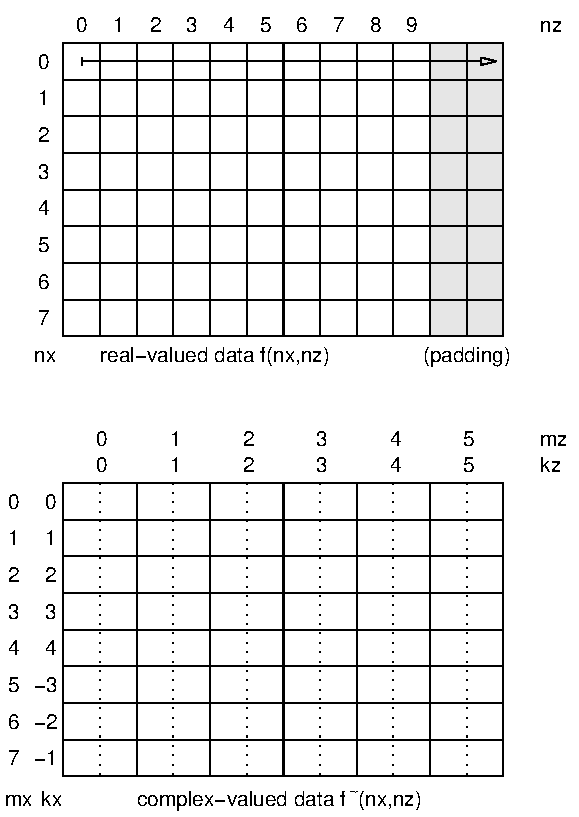
\includegraphics[height=5.0in]{datalayout}
\end{center}
\caption{{\bf Layout of data in memory for real-to-complex $xz$-Fourier transforms}
for the case $N_x = 8$, $N_z = 10$. The Fourier transform converts real-valued
data, above, to complex-valued data, below. Each solid box in the upper picture
is a double-precision real number. Each solid box in the picture below is a
double-precision complex number, with real and imaginary parts separated by a
dashed line. The arrow indicates row-major storage order: successive memory
locations store data with successive {\tt nz}.}
\label{fig:datalayout}
\end{figure}

FlowField's $xz$ memory layout is taken directly from FFTW. Figure
\ref{fig:datalayout} illustrates $xz$ memory layout for the case
$N_x=8$ and $N_z=10$. The upper picture represents an $N_z \times N_x$
array of double-precision real numbers, with two columns for padding.
The bottom picture shows the same memory after the Fourier transform,
now interpreted as an $M_x \times M_z = N_x \times (N_z/2+1)$ array of
complex numbers. In the bottom picture note the correspondence between
the mode-number array index $m_x$ and the wavenumber $k_x$, and the
reduced range of the $m_z$ array index. The Fourier coefficients with
negative $k_z$ are defined implicitly by $\widetilde{f}_{k_x, -k_z} =
\widetilde{f}_{-k_x, k_z}^*$.

%\begin{align}
%\widetilde{f}_{k_x, k_z} &= \frac{1}{N_x N_z} \sum_{n_x=0}^{N_x-1} \sum_{n_z=0}^{N_z-1} f_{n_x, n_z} \: e^{-2 \pi i (k_x n_x/N_x + k_z n_z/N_z)}
%\label{eqn:2d_DFTb} \\
%f_{n_x, n_z} &= \sum_{k_x=-N_x/2}^{N_x/2-1} \; \sum_{k_z=-N_z/2}^{N_z/2-1} \widetilde{f}_{k_x, k_z} e^{2 \pi i (k_x n_x/N_x + k_z n_z/N_z)}
%\label{eqn:2d_IDFTb}
%\end{align}

\subsection{DNS and related classes}
\label{sec:nsintegrator}

A DNS object advances a pair of velocity and pressure FlowFields
forward in time, according to the Navier-Stokes. This section
describes how to use the DNS class. For its mathematical details,
see \Sec{sec:math_details}.

DNS objects are constructed by
\begin{alltt}
  DNS dns(u, U, nu, dt, flags);
\end{alltt}
or
\begin{alltt}
  DNS dns(u, U, nu, dt, flags, T0);
\end{alltt}
Of the arguments, {\tt u} is a FlowField representing the
initial condition of the fluctuating velocity, {\tt U} is a
ChebyCoeff representing the base flow, {\tt dt} is either a
Real number or a TimeStep object representing the finite-difference
time step, and {\tt flags} is a DNSFlags object. The optional
{\tt T0} argument is a real number that specifies the starting time
or the integration.

\subsubsection{Configuring DNS with DNSFlags}
\label{sec:dnsflags}

The DNSFlags class is used to configure some optional generalizations
of CHQZ's algorithm. DNSFlags contains several flag variables which can
be set at construction or assigned afterwards. For example,
\begin{alltt}
  DNSFlags flags(BulkVelocity, CNAB2, Rotational, DealiasXZ, PrintTime);
\end{alltt}
or
\begin{alltt}
  DNSFlags flags; // set to default values
  flags.constraint   = PressureGradient;
  flags.timestepping = CNAB2;
\end{alltt}
The complete set of DNSFlags variables and their allowed values are
\vspace{2mm}

\begin{tabular}{ll}
DNSFlags variable  & allowed values (default first)\\
{\tt flags.constraint}   & {\tt BulkVelocity, PressureGradient}\\
{\tt flags.timestepping} & {\tt CNFE1, CNAB2, CNRK2, SMRK2, SBDF1, ..., SBDF4} \\
{\tt flags.initstepping} & {\tt CNFE1, CNRK2, SMRK2} \\
{\tt flags.nonlinearity} & {\tt Rotational, SkewSymmetric, Alternating, Linearized} \\
{\tt flags.dealiasing}   & {\tt DealiasXZ, NoDealiasing, DealiasY, DealiasXYZ} \\
{\tt flags.verbosity}    & {\tt PrintTime, Silent, VerifyTauSolve, PrintAll}
\end{tabular}
\vspace{2mm}

\noindent
The basic meanings of the DNSFlags variables are
\begin{itemize}
\item {\tt flags.constraint} : Periodic channel flows satisfy the
Navier-Stokes equations with either the bulk velocity or the
spatial-mean pressure gradient set as an external constraint. This
flag sets which constraint is to be enforced. DNS's default
behavior determines the spatial-mean pressure gradient or bulk
velocity from the fluctuation's initial condition {\tt u} and matches
this as a fixed constraint at each time step. DNS can match
time-varying constraints as well. See \Sec{sec:enforcement} for further
details.
\item {\tt flags.timestepping}: The DNS class implements seven different
time-stepping algorithms. (The default is SBDF3.)
\begin{itemize}
  \item {\tt CNFE1} or {\tt SBDF1}: 1st-order Crank-Nicolson, Foward-Euler or
  1st-order Semi-implicit Backward Differentiation Formula --two names for
  the same algorithm. This algorithms is extremely simple and needs no
  initialization need, but its 1st-order error scaling makes it practically
  worthless, except for initializing other algorithms.
  \item {\tt CNAB2} 2nd-order Crank-Nicolson, Adams-Bashforth. A popular
  algorithm, but higher-frequency modes are poorly damped (see \cite{Ascher95})
  Requires one initialization step. Zang warns against using {\tt CNAB2}
  in combination with Rotational nonlinearity unless the high-frequency modes
  are dealiased \cite{Zang95}. {\tt CNAB2} enforces zero-divergence at
  successive timesteps and momentum equations halfway between successive
  time steps, which can lead to slowly decaying period-$2dt$ oscillation
  in the pressure field, unless pressure and velocity are initialized
  accurately.
  \item {\tt CNRK2}: a three-substep, 2nd-order semi-implicit Crank-Nicolson,
  Runge-Kutta algorithm, developed by Zang and Hussaini \cite{Zang95} and
  but implemented in Channelflow from the Peyret's exposition \cite{Peyret02}.
  According to Peyret, Zang and Hussaini observed 3rd-order scaling for
  this algorithm applied to low-viscosity flows, even though it is
  theoretically 2nd-order. Numerical tests in Channelflow show 2nd-order
  scaling for velocity fields at $\Rey = 10^3 - 10^4$, and {\em 1st-order}
  scaling for pressure, due to a phase error in the pressure field. {\tt CNRK2}
  requires no initialization.
  \item {\tt SMRK2}: a three-substep, 2nd-order semi-implicit Runge-Kutta
  developed by Spalart, Moser, and Rogers \cite{Spalart91}. Identical
  characteristics as {\tt CNRK2}, including observed 2nd-order scaling
  consistent with theory, contrary to authors' claim of 3rd-order scaling,
  and 1st-order phase error in pressure. Requires no initialization.
  \item {\tt SBDF2, SBDF3, SBDF4}: 2nd, 3rd, and 4th-order Semi-implicit
  Backward Differentiation Formulae, requiring 1,2, and 3 initialization
  steps. I have found the {\tt SBDF} schemes to be the best-behaved of the
  lot. When solving $u^{n+1}$ and $p^{n+1}$, {\tt SBDF} schemes enforce
  divergence and momentum equations at $t_{n+1}$. This strongly implicit
  formulation poduces strong damping for high-frequency modes and results
  in pressure field as accurate as the velocity field. {\tt SBDF3} is
  particularly good: it has the strongest asympotitc decay of all 3rd-order
  implicit-explicit linear multistep schemes. For these reasons, {\tt SBDF3}
  is the default value of {\tt flags.timestepping}.
    Peyret terms these algorithms AB/BDEk ($k$th-order Adams-Bashforth
  Backward-Differentiation).
\end{itemize}
\item {\tt flags.initstepping}: Some of the time-stepping algorithms listed
above ({\tt SBDF} in particular) require data from N previous time steps.
Supplying these past values to the DNS constructor would entail a number
of tedious practical problems, so the DNS class instead takes its first N
steps with an {\em initialization timestepping} algorithm that
requires no previous data. This initialization algorithm is specified by
{\tt flags.initstepping}. Valid values are {\tt CNFE}, {\tt CNRK2}, and
{\tt SMRK2}. The default is {\tt CNRK2}.
\item {\tt flags.nonlinearity}: The nonlinear term in the Navier-Stokes
calculation can be computed in a number of forms that are equivalent in
continuous mathematics but slightly different when computed with spectral
expansions and collocation. The default is {\tt SkewSymmetric}.
\begin{itemize}
  \item {\tt Rotational}: Fast but generates high-frequency errors unless
  dealiased (see \cite{Zang91}).
  \item {\tt SkewSymmetric}: Comparatively expensive to compute (factor of
  two (?) compared to {\tt Rotational} but
  \item {\tt Convective}.
  \item {\tt Divergence}.
  \item {\tt Alternating} convection/divergence an alternating time steps.
  A cheap approximation to {\tt SkewSymmetric}, which is an average of
  the convective and divergence forms. I have not yet analyzed how the
  alternating nonlinearity method interacts with multistepping algorithms.
  \item {\tt Linearized} about the base flow.
\end{itemize}
\item {\tt flags.dealiasing}: Nonlinear terms are calculated with
collocation methods. FlowFields can be padded with zeros to
eliminate aliasing errors. {\tt DealiasXZ} causes 2/3-style padding
in $xz$: at each time-step the upper 1/3 of $x$ and $z$ of the velocity
field's Fourier coefficients are set to zero. Eventually, {\tt DealiasY}
will cause 3/2-style padding in $y$, with collocation calculations performed
in temporary arrays of length $3 N_y/2$ --but that is not yet implemented!
See \cite{Canuto88} and  \Sec{sec:timestep_algorithms} for more details.
\item {\tt flags.verbosity}: This flag governs what the DNS prints
at each timestep. {\tt PrintTime} prints the integration time at each
timestep, which is helpful when running Channelflow programs interactively.
{\tt VerifyTauSolve} prints a verbose and expensive verification of the
tau-equation solutions for each Fourier mode. Other values are
self-explanatory.
\end{itemize}

For precise specification of how the DNSFlags configuration variables
affect the integration, please refer to \Sec{sec:math_details}.

\subsubsection{Base-fluctuation decomposition}

DNS decomposes the velocity and pressure fields into {\em base} and
{\em fluctuating} parts in the form
\begin{align}
\bu_{\text{tot}}(\bx,t) &= U(y) \be_x + \bu(\bx,t) \label{udecomp}\\
\ptot(\bx,t)  &= x \frac{dP}{dx}(t) + p(\bx,t)     \label{pdecomp}
\end{align}
Channelflow represents the fluctuating velocity and pressure fields
$\bu$ and $p$ with $xz$-periodic FlowFields. Hence in the decomposition
of the pressure gradient,
\begin{align}
\grad \ptot(\bx,t)  &= \frac{dP}{dx}(t) \be_x + \grad p(\bx,t),
\end{align}
the fluctuating pressure gradient $\grad p$ has a zero spatial mean,
and all of the spatial-mean pressure gradient is carried by the base
pressure gradient. For simplicity, $dP/dx$ is referred to as the
mean pressure gradient in subsequent material, with spatial-mean
implied. DNS imposes no further restriction on the
base flow $U(y)$ or the base pressure gradient $dP/dx$: they do not
have to solve the Navier-Stokes equations as a pair, nor is $\bu$
required to have zero spatial mean. The base flow $U(y)$ for a
simulation is set through the ChebyCoeff {\tt U} argument to the
DNS constructor.

\subsubsection{Enforcing bulk velocity or mean pressure constraints}
\label{sec:enforcement}

A channel flow can satisfy either an externally imposed bulk velocity,
or an externally imposed mean pressure gradient. When one of
is enforced as a constraint, the other is a dependent variable whose
value is determined from the momentum equation. The DNS class allows
either type of constraint, as specified by its DNSFlags argument.
By default, the DNS determines the value of the constraint from
the initial data and matches that value at all future times. For bulk
velocity, the initial value is determined by
\begin{align}
U_{\text{bulk}} = \frac{1}{L_x L_z (b-a)} \int_0^{L_x} \int_a^b \int_0^{L_z}
U(y) + u(\bx,0) \; dx \; dy \; dz
\end{align}
The initial mean pressure gradient is set from the initial
wall-shear, according to
\begin{align}
 \frac{dP}{dx} = \frac{\nu}{b-a}
\left( \frac{du_{\text{mean}}}{dy} \bigg\vert_b -
 \frac{du_{\text{mean}}}{dy} \bigg\vert_a \right) \label{dPdx_init}
\end{align}
{\em Check correctness of eqn, use of $\nu$ vs $\mu$, and $\rho$.}
Note that this choice is somewhat arbitrary --it assumes the net
acceleration of the fluid is zero.

The DNS class allows the initial constraint values to be reset. For example,
\begin{alltt}
  DNS dns(u,U,nu,dt,flags);
  dns.reset\_dPdx(0.0);
\end{alltt}
resets the mean pressure constraint to zero and sets the constraint type
to {\tt PressureGradient}.
\begin{alltt}
  DNS dns(u,U,nu,dt,flags);
  dns.reset\_Ubulk(0.0);
\end{alltt}
resets the bulk velocity constraint to zero and sets the constraint type
to {\tt BulkVelocity}.

\subsubsection{Fixed and variable time-stepping}
\label{sec:fixed_variable_timestepping}

\subsubsubsection{Fixed time-stepping}

In the simplest case, a DNS performs fixed time-stepping and
enforces a constant bulk velocity or mean pressure gradient
\begin{alltt}
   Real dt=0.10;
   DNSFlags flags(BulkVelocity, RK3, Rotational, DealiasXZ, PrintTime);
   DNS dns(u, U, nu, dt, flags);

   for (int n=0; n<N; ++n)
      dns.advance(u, q);
\end{alltt}
The loop advances the fluctuating velocity {\tt u} and modified pressure
{\tt q} {\tt N} steps of length {\tt dt}. The {\tt advance()} function
can also take multiple steps internally, for example,
\begin{alltt}
   int m = 10;
   for (int n=0; n<N; ++n)
      dns.advance(u, q, m);
\end{alltt}
advances {\tt u} and {\tt q} a total of {\tt N*m} steps of length {\tt dt}.
The integration time can be determined at any point by calling
{\tt Real t = dns.advance(u, q, m);}.

\subsubsubsection{Variable time-stepping}

Variable time-stepping minimizes the computational cost of an integration
by maximizing the timestep while keeping the CFL number near a threshold.
The optional TimeStep class automates some of the issues associated with
variable timesteps. TimeStep tries to maximize the CFL number subject to
the constraints that (1) the timestep stays in a given range, (2) the CFL
number stays in a given range, and (3) the timestep is a whole-number
fraction of a fixed time-interval. The last constraint allows one to
stop and examine integrations at fixed time-intervals. For example,
\begin{alltt}
   TimeStep dt(dtstart, dtmin, dtmax, dT, CFLmin, CFLmax);
   DNS dns(u, U, nu, dt, flags);

   for (Real t=0; t<T0; t += dT) \{
     dns.advance(u, q, dt.n());

     if (dt.adjust(dns.CFL()))
       dns.reset(nu, dt);
   \}
\end{alltt}
In this example, the TimeStep object adjusts itself to keep the
CFL number between {\tt CFLmax} and over {\tt CFLmin}, {\tt dt}
between {\tt dtmin} and {\tt dtmax}, and {\tt dt} a whole-number
fraction of {\tt dT}, so that {\tt dt*dt.n() = dT} and each pass
through the for-loop then covers the same time-interval. If the
CFL number goes out of range, {\tt dt.adjust} changes the value
of the time step and returns {\tt true}, and the {\tt dns}
object is reset to compute with the new integration timestep.
Resetting the DNS's timestep is a moderately expensive
operation (about the same as advancing one timestep), so it
should be done infrequently.

Note that, when using {\tt CNAB2} or {\tt SBDF} (multistep) time-stepping
algorithms, resetting the time step requires reinitializing the multistep
algorithm. In this case, the DNS object reinitialize by taking several
steps with the {\tt flags.initstepping} algorithm.

{\em CFL number. Measure expense of dns.reset().}

\subsubsubsection{Time-varying constraints}

The following code enforces a time-varying bulk velocity.
\begin{alltt}
   DNSFlags flags;
   flags.constraint = BulkVelocity;
   DNS dns(u, U, nu, dt, flags);
   for (Real t=0; t<T0; t += dt) \{
     Real ubulk = sin(k*t);
     dns.advance(u, q, ubulk);
   \}
\end{alltt}
To enforce a time-varying constraint on the pressure gradient,
change the first DNSFlags argument to {\tt PressureGradient} and
rename {\tt ubulk} to {\tt dPdx} for clarity.

Note that time-varying constraints require CNAB2 time-stepping.
I haven't yet figured out how to enforce the constraints properly
in RK3 substeps. Note also that the {\tt advance} function distinguishes
variable-constraint timestepping from multistep time-stepping
(\Sec{sec:fixed_variable_timestepping} by the type of the third argument.
If you write
\begin{alltt}
   Real m = 10;             // note the Real type
   for (int n=0; n<N; ++n)
      dns.advance(u, q, m); // enforce Ubulk or dPdx to 10!
\end{alltt}
{\tt advance()} will interpret the {\tt m} argument as a time-varying
constraint to be enforced!

\section{Mathematical details}
\label{sec:math_details}

This section discusses in some detail the mathematics of the
spectral Channelflow algorithm, in order to specify the consequences
of configuration choices and to provide a point of reference for
comments in the source code.

\subsection{The Navier-Stokes equations}
\label{sec:NSeqns}

\begin{figure}
%\vspace{3.0in}
%\usepackage[dvips]{graphics}
\centering
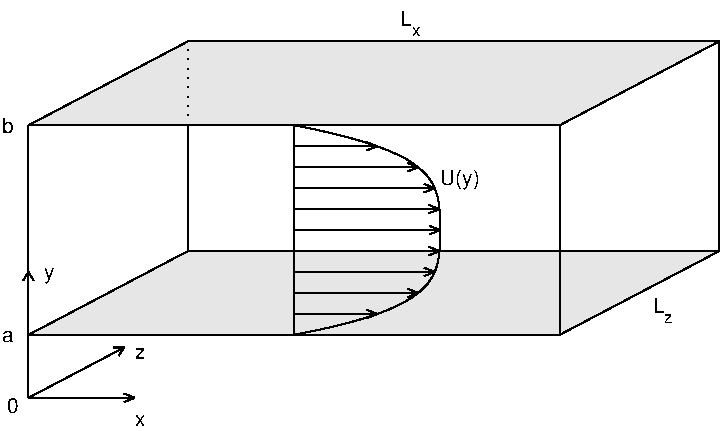
\includegraphics[height=2.0in]{schematic}
\caption{{\bf Schematic of channel flow.} Fluid flows between
two rigid walls at $y=a$ and $y=b$. The boundary conditions are
periodic in $x$ and $z$ and no-slip at the walls. The mean flow $U(y)$
is driven in the $x$-direction by a mean pressure gradient.}
\label{schematic}
\end{figure}

Consider an incompressible wall-bounded fluid flow in a rectangular
domain $\Omega \defn L_x \mathbb{T} \times [a, b] \times L_z \mathbb{T}$,
where $\mathbb{T}$ is the periodic unit interval. The fluid flow in
$\Omega$ is governed by the incompressible Navier-Stokes equations,
\begin{align}
\frac{\del \butot}{\del t} + \butot \cdot \bnabla \butot & = -  \bnabla \ptot + \nu \lapl \butot \label{NS0a} ,\\
\dvrg \butot & = 0, \label{NS0b}
\end{align}a
where $\butot(\bx,t)$ is the total fluid velocity field and
$\ptot(\bx,t)$ is the total pressure field. The upper and lower
surfaces of $\Omega$ are rigid walls, giving rise to no-slip boundary
conditions: $\bu = 0$ at $y=a$ and $y=b$. The boundary conditions in
the $x$ and $z$ directions are periodic: $\butot(x+L_x,y,z,t) =
\butot(x,y,z,t)$ and $\butot(x,y,z+L_z,t) =
\butot(x,y,z,t)$.\footnote{Components of vector variables are written
several ways: $\bx = (x,y,z)$ or $\bx=(x_0,x_1,x_2)$, and $\bu = (u,v,w)$
or $(u_0, u_1, u_2)$. A unit vector in the $x$ (or $x_0$) direction is
$\be_x$ (or $\be_0$).}

\subsection{Base-fluctuation decomposition}
\label{sec:basefluc}

Channelflow allows the total velocity and pressure fields to be broken
into constant and fluctuating parts. The velocity field is the sum of
the {\em base velocity} or {\em base flow} $U(y) \be_x$, and the
{\em fluctuating velocity} $\bu(\bx,t)$.
\begin{align}
\butot(\bx,t) &= U(y)\: \be_x + \bu(\bx,t). \label{eqn:udecomp}
\end{align}
The total pressure field is the sum of a linear-in-$x$ term $\Pi_x(t)
\: x$ and a periodic fluctuating pressure $p(\bx,t)$. The gradient of
this decomposition relates the total pressure gradient to a
spatially-constant {\em base pressure gradient} $\Pi_x \be_x$ and a
{\em fluctuating pressure gradient} $\grad p(\bx,t)$.
\begin{align}
\ptot(\bx,t)  &= \Pi_x(t)\: x + p(\bx,t) \\
\grad \ptot(\bx,t)  &= \Pi_x(t) \:\be_x + \grad p(\bx,t) \label{eqn:gradpdecomp}
\end{align}
These forms for the base flow and pressure gradient are general enough
to represent cases like Poisseuille, Couette, and turbulent
mean profiles. Note that Channelflow does not require the base velocity
and base pressure gradient to satisfy the Navier-Stokes equations themselves.
Substituting \eqns{eqn:udecomp}{eqn:gradpdecomp} into \eqn{NS0a} gives
\begin{align}
\frac{\del \bu}{\del t} +  \grad p = \nu \lapl \bu - \butot \cdot \grad \butot + \left[\nu  \frac{\del^2 U}{\del y^2} - \Pi_x \right] \be_x \label{NS1a}
\end{align}


\subsection{Forms for the nonlinear term}
\label{sec:nonlinearity}

There are several  different forms for the term of form $\butot \cdot \grad \butot$
in \eqn{NS1a} that are identical in continuous mathematics but have different
properties when discretized. These are
\begin{align}
\text{{\em the convection form }} & \quad \butot \cdot \grad \butot \\
\text{{\em the divergence form }} & \quad \grad \cdot(\butot \butot) \\
\text{{\em the skew-symmetric form }} & \quad \frac{1}{2} \butot \cdot \grad \butot  + \frac{1}{2} \grad \cdot (\butot \butot) \\
\text{{\em the rotational form }} & \quad (\nabla \cross \butot) \cross \butot + \frac{1}{2} \grad (\butot \cdot \butot)
\end{align}
These expressions are identically equal, assuming $\grad \cdot \butot
= 0$. When discretized, the rotational form is the least expensive to
compute, but it introduces errors in the high spatial frequencies
unless dealiased transforms are used. The skew-symmetric form produces
no such errors but is roughly twice as expensive to compute. Note that
the skew-symmetric form is the average of the convection and
divergence forms. One can simulate this averaging by alternating
between the convection and divergence forms on successive timesteps.
In practice the alternating method is as well-behaved as the
skewsymmetric and almost as fast as the rotational. Zang recommends
using the skew-symmetric or alternating forms with aliased transforms
or the rotational form with dealiased transforms. See Zang
(\cite{Zang91}) for further details. Channelflow implements the
rotational, convection, divergence, skew-symmetric, and alternating
forms. The form is chosen by setting the DNSFlags {\tt nonlinearity}
variable --see
\Sec{sec:dnsflags}.

For historical reasons, the Channelflow does not compute the rotational
form exactly as shown above; rather, the nonlinear term is first expanded
with the base-fluctuation decomposition and then the rotational form is
applied to $\bu \cdot \grad \bu$:
\begin{align}
\butot \cdot \grad \butot &= U \frac{\del \bu}{\del x} + v \frac{\del U}{\del y} \be_x + \bu \cdot \grad \bu  \\
&= U \frac{\del \bu}{\del x} + v \frac{\del U}{\del y} \be_x + (\nabla \cross \bu) \cross \bu + \frac{1}{2} \grad (\bu \cdot \bu)
\end{align}

DNS computes the nonlinear term according to the value of
{\tt flags.nonlinearity}. Here we list the form of the Navier-Stokes
equation solved by DNS with various values of the flags
(with $\butot = \bu + U \be_x$ and $U$ fixed).

\noindent
Rotational:
\begin{align}
\frac{\del \bu}{\del t} + \grad \left[ p + \frac{1}{2} \bu \cdot \bu \right]
&= \nu \lapl \bu - \left[ (\nabla \cross \bu) \cross \bu + U \frac{\del \bu}{\del x} + v \frac{\del U}{\del y} \be_x \right] + \left[\nu  \frac{\del^2 U}{\del y^2} - \Pi_x \right] \be_x \label{NS1a_rotational}
\intertext{Convection:}
\frac{\del \bu}{\del t} + \grad  p
&= \nu \lapl \bu -  \butot \cdot \grad \butot  + \left[\nu  \frac{\del^2 U}{\del y^2} - \Pi_x \right] \be_x \label{NS1a_convection}
\intertext{Divergence:}
\frac{\del \bu}{\del t} + \grad  p
&= \nu \lapl \bu - \grad (\butot \cdot \butot)  + \left[\nu  \frac{\del^2 U}{\del y^2} - \Pi_x \right] \be_x \label{NS1a_divergence}
\intertext{Skew-symmetric:}
\frac{\del \bu}{\del t} + \grad  p
&= \nu \lapl \bu - \left[\frac{1}{2} \butot \cdot \grad \butot + \frac{1}{2} \grad (\butot \cdot \butot) \right] + \left[\nu  \frac{\del^2 U}{\del y^2} - \Pi_x \right] \be_x \label{NS1a_skewsymm}
\intertext{Linearized:}
\frac{\del \bu}{\del t} + \grad  p
&= \nu \lapl \bu - \left[ U \frac{\del \bu}{\del x} + v \frac{\del U}{\del y} \be_x \right] + \left[\nu  \frac{\del^2 U}{\del y^2} - \Pi_x \right] \be_x \label{NS1a_linearized}
\end{align}
Alternating: eqns.\ \ref{NS1a_convection} and \ref{NS1a_divergence} on alternating time steps.

Eqns.\ \ref{NS1a_skewsymm}-\ref{NS1a_linearized} can be reunited with
notation. With $U$ fixed and $\butot$ defined as $\bu + U \be_x$, define the
{\em nonlinear term} $\bN(\bu)$ by
\begin{align}
\bN(\bu) &\defn
\begin{cases}
(\nabla \cross \bu) \cross \bu + U \frac{\del \bu}{\del x} + v \frac{\del U}{\del y} \be_x
& \text{Rotational} \\
\butot \cdot \grad \butot  & \text{Convection} \\
\frac{1}{2} \grad (\butot \cdot \butot)  & \text{Divergence} \\
\frac{1}{2} \butot \cdot \grad \butot  + \frac{1}{2} \grad (\butot \cdot \butot)  & \text{Skew-symmetric} \\
U \frac{\del \bu}{\del x} + v \frac{\del U}{\del y} \be_x & \text{Linearized} \label{N_defn}
\end{cases}
\end{align}
and the {\em modified pressure} $q$ by
\begin{align}
q &\defn
\begin{cases}
 p + \frac{1}{2} \bu \cdot \bu & \text{Rotational} \\
 p & \text{else} \\
\label{q_defn}
\end{cases}
\end{align}
Define also the {\em linear term} $\bL(\bu)$ and the
{\em constant term} $\bC$ by
\begin{align}
\bL \bu &\defn \nu \lapl \bu \\
\bC &\defn \left[ \nu  \frac{\del^2 U}{\del y^2} - \Pi_x \right] \be_x
\end{align}
Note that the constant term is constant in $\bu$, but it may vary in
time, since it contains the mean pressure gradient, which is a
potentially time-varying external forcing parameter. With these
definitions \eqns{NS1a_skewsymm}{NS1a_rotational} can be written
\begin{align}
\frac{\del \bu}{\del t} + \grad q = \bL \bu  - \bN (\bu) + \bC \label{NS2a}
\end{align}
The DNS {\tt advance(u,q)} function advances the FlowFields
{\tt u} and {\tt q} to their (approximate) values at the next time step,
according to \eqn{NS2a} and the constraint $\grad \cdot\bu = 0$. Note
that the meaning of the returned value of {\tt q} depends on the
choice of nonlinearity, according to \eqn{q_defn}.

The next step in the derivation is to Fourier-transform \eqn{NS1a}.
We apply the continuous Fourier transform (\eqn{eqn:2d_FT}) since
\eqn{NS1a} is continuous and introduce truncation later.
The Fourier-transformed operators for the gradient, the Laplacian,
and the linear operator $\bL$ are
\begin{align}
\tgrad_{k_x k_z} &\defn 2 \pi i \frac{k_x}{L_x} \be_x + \frac{\del}{\del y} \be_y  + 2 \pi i \frac{k_z}{L_z} \be_z \label{tgrad}, \\
\tlapl_{k_x k_z} &\defn \frac{\del^2}{\del y^2}  - 4 \pi^2 \left(
\frac{k_x^2}{L_x^2} + \frac{k_z^2}{L_z^2}\right), \\
\tbL_{k_x k_z} &\defn \nu \tlapl_{k_x k_z}
\end{align}
With these definitions, $\widetilde{\grad q} = \tgrad \tq$ and
$\widetilde{\bL \bu} = \tbL \tbu$. Here and onwards $k_x k_z$
subscripts will often be suppressed, to reduce clutter. The Fourier
transform of \eqn{NS1a} can then be written
\begin{align}
\frac{\del \tbu}{\del t} + \tgrad \tq = \tbL \tbu - \widetilde{\bN(\bu)} + \tbC \label{NS3a}
\end{align}
Note that since $\bC$ is spatially constant, so
${\tbC} = \bC \: \kron_{k_x 0} \: \kron_{k_z 0}$.



\subsection{Time-stepping algorithms}
\label{sec:timestep_algorithms}

DNS currently offers two time-integration schemes: CNAB2,
a mixed Crank-Nicolson/Adams-Bashforth scheme, and RK3, a mixed
3rd-order Runge-Kutta scheme. Both schemes treat the linear term
implicitly and the nonlinear term explicitly. CNAB is simpler so
let's begin there. Let $\tbu^n$ be the approximation of $\tbu$
at time $t=n \Delta t$, and let $\tbN^n \defn \widetilde{\bN(\bu^n)}$.
Then we approximate terms in \eqn{NS3a} at $t = (n-1/2) \Delta t$ with
\begin{align}
\frac{\del}{\del t} \tbu^{n+1/2} &= \frac{\tbu^{n+1} - \tbu^{n}}{\Delta t} + O(\Delta t^2) \\
 \tbL \tbu^{n+1/2} &= \frac{1}{2} \tbL \tbu^{n+1} + \frac{1}{2} \tbL \tbu^{n} + O(\Delta t^2) \\
 \tgrad \tq^{n+1/2} &= \frac{1}{2} \tgrad \tq^{n+1} + \frac{1}{2} \tgrad \tq^{n} + O(\Delta t^2) \\
 \tbN^{n+1/2} &= \frac{3}{2} \tbN^{n} \:\:\:\:\:\: - \frac{1}{2} \tbN^{n-1} + O(\Delta t^2) \\
 \tbC^{n+1/2} &= \frac{1}{2} \tbC^{n+1} \:\: + \frac{1}{2} \tbC^{n} + O(\Delta t^2)
\end{align}
The time-derivative approximation is obvious, the approximation for the
linear term is called Crank-Nicolson, and that of the nonlinear term is
Adams-Bashforth (see CHQZ section 4.3). Plugging those into \eqn{NS3a}
and rearranging gives
\begin{align}
\left[ \frac{1}{\Delta t} - \frac{1}{2} \tbL\right] \tbu^{n+1} + \frac{1}{2} \tgrad q^{n+1}
= \left[ \frac{1}{\Delta t} + \frac{1}{2} \tbL\right] \tbu^{n} - \frac{1}{2} \tgrad q^n
+ \frac{3}{2} \tbN^{n} - \frac{1}{2} \tbN^{n-1} + \frac{1}{2} \tbC^{n+1} + \frac{1}{2} \tbC^{n} \label{CNAB}
\end{align}
At this point we drop the $O(\Delta t^2)$ notation and take \eqn{CNAB}
as an update rule for an approximate solution $\tbu^{n+1}$. \Eqn{CNAB}
has several notable properties: (1) it is linear in the unknowns
$\tbu^{n+1}$ and $\tq^{n+1}$, (2) its right-hand side can be computed
directly from velocity and pressure fields at previous time-steps and the
external mean-pressure parameter, and (3) the linear equations for each
Fourier mode $k_x k_z$ are independent.

Channelflow's 3rd-order Runge-Kutta scheme, based on \cite{Spalart91},
is similar in principle but involves three substeps for each timestep
of length $\Delta t$, with different coefficients $\alpha_i$, $\beta_i$,
$\gamma_i$, and $\zeta_i$ for each substep.
\begin{multline}\label{RK3}
\left[\frac{1}{\Delta t} - \beta_i\tbL\right] \tbu^{n,i+1} + \beta_i \tgrad \tq^{n,i+1} \\
=  \left[\frac{1}{\Delta t} + \alpha_i \tbL\right] \tbu^{n,i} - \alpha_i \tgrad \tq^{n}
+ \gamma_i \tbN^{n,i} + \zeta_i \tbN^{n,i-1}
+ \beta_i  \tbC^{n+1} + \alpha_i \tbC^{n}
\end{multline}
The second superscript indicates the Runge-Kutta substeps. For example,
a three-substep follows the sequence $\tbu^{n,0}, \tbu^{n,1},  \tbu^{n,2},
\tbu^{n+1,0}$. RK3 is a particularly convenient time-stepping scheme because
$\zeta_0=0$ eliminates the previous-step nonlinear term
$\tbN^{n,i-1}$ when $i=0$. Consequently the time-stepping can be
started from a single instantaneous velocity field. For CNAB, both
$\tbN^{n}$ and $\tbN^{n-1}$ are always required, so two consecutive
velocity fields are needed for starting the time-stepping. The CNAB
time-stepping algorithm can also be expressed in a form like \eqn{RK3},
so we'll proceed using this as the general form.

\begin{table}
\centering
\caption{{\bf Time-stepping coefficients}}
\label{rk3coeffs}
\begin{tabular}{l|rcccc}
    & $i$ &	$\alpha_i$ &	$\beta_i$ & $\gamma_i$ & $\zeta_i$ \\\hline
CNAB &0& 1/2 & 1/2 & 3/2 & -1/2 \\\hline
    & 0   & 29/96 & 37/160 & 8/15 & 0 \\
RK3 &1   & -3/40 & 5/24   & 5/12 & -17/60 \\
    &2   & 1/6   & 1/6    & 3/4  & -5/12
\end{tabular}
\end{table}

Expanding $\tbL$ on the left-hand side of \eqn{RK3} results in an equation
of the form
\begin{align}
\nu \tbu''^{\; n,i+1} - \lambda \tbu^{\: n,i+1} - \tgrad \tq^{n,i+1} = -\tbR^{n,i} \label{tau_eqn}
\end{align}
where
\begin{align}
\lambda &\defn \frac{1}{\beta_i \Delta t} + 4 \pi^2 \nu \left(\frac{k_x^2}{L_x^2} + \frac{k_z^2}{L_z^2}\right) \label{lambda_defn} \\
\tbR^{n,i} &\defn \left[ \frac{1}{\beta_i \Delta t} + \frac{\alpha_i}{\beta_i} \tbL\right] \tbu^{n,i} + \frac{\alpha_i}{\beta_i} \tgrad \tq^{n,i} + \frac{\gamma_i}{\beta_i} \tbN^{n,i} + \frac{\zeta_i}{\beta_i} \tbN^{n,i-1} + \tbC^{n,i+1} + \frac{\alpha_i}{\beta_i} \tbC^{n,i} \label{Rdefn} \\
\tbu'' &\defn \frac{d^2}{dy^2} \tbu
\end{align}

Thus, at each timestep or substep, we need to solve \eqn{tau_eqn} for
each Fourier mode. The complete system of equations to be solved is
\begin{align}
\nu \tbu'' - \lambda \tbu - \tgrad \tq & = -\tbR \label{tau_eqn_0a}\\
\tgrad \cdot \tbu &= 0 \label{tau_eqn_0b} \\
\tbu(a) = \tbu &= 0 \label{tau_eqn_0c}
\end{align}
From here on the time superscripts are suppressed. For lack of a better
term, we call eqns.\ \ref{tau_eqn_0a}--\ref{tau_eqn_0c} the
{\em tau equations}. The name derives from the need to add a
{\em tau correction} to the solution of the equations in their
discretized form. See CHQZ Section 7.3.1 and \Sec{sec:tau_correction}.

The bulk of the DNS {\tt advance()} method is concerned with looping
over the Fourier modes and calculating $\tbR$ in preparation for
solving the tau equations. The actual solution is computed by
TauSolver and related classes, discussed in \Sec{sec:tausolver}. If
$xz$-dealiasing is set in the DNSFlags, this loop excludes the highest
one-third of Fourier modes and sets those modes to zero.

\subsection{TauSolver}
\label{sec:tausolver}

The TauSolver class solves equations of the form of
eqns.\ \ref{tau_eqn_0a}--\ref{tau_eqn_0c}. An DNS object
contains an $N_x \times (N_z/2+1)$ array of TauSolvers, each one
configured solving eqns.\ \ref{tau_eqn_0a}--\ref{tau_eqn_0c} for
a given $k_x,k_z$ pair. The TauSolver's solution method is as follows.

\subsubsection{The influence-matrix method.}
\label{sec:influence_matrix}

Eqns.\ \ref{tau_eqn_0a}--\ref{tau_eqn_0c} constitute three coupled
differential equations in four unknowns $(\tu,\tv,\tw,\tq)$, with
one constraint equation and three boundary conditions. CHQZ, following
Klieser and Schumann (\cite{Kleiser80}), show how to decompose these
coupled equations into independent one-dimensional Helmholtz
equations. For simplicity of presentation in this section we assume
the walls are at $y=\pm1$. We can isolate a system of equations in
$\tq$ and $\tv$ by taking the divergence of
\eqn{tau_eqn_0a}, the $\tv$-component of the same, and evaluating
$\tgrad \cdot \tbu = 0$ at the two walls. This gives
\begin{alignat}{2}
\tq'' - \kappa^2 \tq &= - \tgrad \cdot \tbR \qqquad & \tv'(\pm 1) &= 0 \label{q_A} \\
\nu \tv'' - \lambda \tv - \tq\;' &= -\hR_y & \tv(\pm 1) &= 0 \label{v_A}
\end{alignat}
Eqns.\ \ref{q_A} and \ref{v_A} form a complete system for $\tq$ and
$\tv$. Call this the {\em A-problem}. The A-problem is tricky to
solve because $\tq$ appears in the $\tv$ differential equation while
$\tv$ appears in the boundary condition.

To solve the A-problem, consider the inhomogeneous {\em B-problem}:
\begin{alignat}{2}
\tq'' - \kappa^2 \tq &= - \tgrad \cdot \tbR  \qqquad & \tq(\pm 1) &= Q_{\pm} \label{q_B} \\
\nu \tv'' - \lambda \tv - \tq\;' &= -\hR_y & \tv(\pm 1) &= 0 \label{v_B}
\end{alignat}
The proper values $Q_{\pm}$ for the modified-pressure boundary conditions
are unknown but will be determined from the requirement that $
\tv'(a) = \tv'(b) = 0$. First let $(\tq_p, \tv_p)$ be the particular
solution to the A-problem with homogeneous Dirichlet boundary conditions,
i.e.
\begin{alignat}{2}
\tq_p'' - \kappa^2 \tq_p &= - \tgrad \cdot \tbR \qquad
& \tq_p(\pm 1) &= 0 \label{q_p} \\
\nu \tv_p'' - \lambda \tv_p - \tq_p' &= -\hR_y
& \tv_p(\pm 1) &= 0 \label{v_p}
\end{alignat}
Next solve the {\em $B_+$-problem},
\begin{alignat}{2}
\tq_+'' - \kappa^2 \tq_+ &= 0 \qqquad
& \tq_+(-1) &= 0, \quad \tq_+(1)= 1\label{q_B+} \\
\nu \tv_+'' - \lambda \tv_+ - \tq_+' &= 0
& \tv_+(\pm 1) &= 0 \label{v_B+}
\end{alignat}
and the {\em $B_-$-problem},
\begin{alignat}{2}
\tq_-'' - \kappa^2 \tq_- &= 0 \qqquad
& \tq_-(-1) &= 1, \:\:\:\: \tq_-(1) = 0\label{q_B-} \\
\nu \tv_-'' - \lambda \tv_- - \tq_-' &= 0
& \tv_-(\pm 1) &= 0 \label{v_B-}
\end{alignat}

Then the solution to the A-problem can be formed from the solutions to
the particular A-problem and the homogeneous $B_{\pm}$-problems, by
\begin{align}
\binom{\tq}{\tv} = \binom{\tq_p}{\tv_p} + \delta_+ \binom{\tq_+}{\tv_+} + \delta_-\binom{\tq_-}{\tv_-}, \label{A_solution}
\end{align}
The boundary conditions on $(\tq, \tv)$ for the A-problem are
satisfied if
\begin{align}
\begin{bmatrix}
\tv_+'(+1) & \tv_-'(+1) \\
\tv_+(-1) & \tv_-(-1)
\end{bmatrix}
\begin{pmatrix} \delta_+  \\ \delta_- \end{pmatrix}
=
- \begin{pmatrix} \tv_p(+1)  \\ \tv_p(-1) \end{pmatrix}
\label{influence_matrix}
\end{align}
\Eqn{influence_matrix} is known as the {\em influence-matrix} equation.
Solving it for $\delta_{\pm}$ produces the proper boundary conditions
for the B-problem, and the consequent solution to the B-problem then
satisfies the original A-problem. Alternatively, one can construct the
solution to the A-problem directly from \ref{A_solution}. Note that
the $B_{\pm}$-problems are independent of the velocity and pressure
fields, so their solutions can be precomputed and stored. This saves
two complex Helmholtz computations per timestep for each Fourier mode.
Channelflow takes this approach. An alternative is to determine boundary
conditions $\tq(\pm 1)=Q_{\pm}$ from $\delta_{\pm}$ and \eqn{A_solution}, and
use this to solve \eqns{q_B}{v_B}. This would save memory at the expense
two complex Helmholtz solutions per timestep. In the future Channelflow
might allow this as an option.

%\begin{align}
%\nu \tu'' - \lambda \tu - \frac{2\pi i k_x}{L_x} \tq &= -\hR_x
%\:\:\:\:\:\:\:\:\:\:\:\:\tu(\pm 1) = 0 \label{u_A} \\
%\nu \tv'' - \lambda \tv - \tq\;' &= -\hR_y
%\:\:\:\:\:\:\:\:\:\:\:\:\tv(\pm 1) = 0 \label{v_AA} \\
%\nu \tw'' - \lambda \tw - \frac{2\pi i k_z}{L_x} \tq &= -\hR_z
%\:\:\:\:\:\:\:\:\:\:\:\:\tw(\pm 1) = 0 \label{w_A}
%\end{align}


\subsubsection{The tau correction}
\label{sec:tau_correction}

To be written.

\subsection{HelmholtzSolver}
\label{sec:helmholtzsolver}

The differential equations to be solved in \Sec{sec:tausolver} are all
Helmholtz equations of the form
\begin{align}
\nu u'' - \lambda u = f
\qquad u(\pm 1) &= u_{\pm} \label{helmholtz_form}
\end{align}
where $u$ is unknown, $\nu$ and $\lambda$ are given parameters, and the
right-hand-sides $f$ and $u_{\pm}$ are given. The Chebyshev tau approximation
of \eqn{helmholtz_form} is
\begin{align}
\nu \hat{u}_n^{(2)} - \lambda \hu_n & = \hf_n  \quad 0 \leq n \leq N-3 \label{u2n} \\
\sum_{n=0}^{N-1} \hu_n &= u_{+} \label{u_bc0} \\
\sum_{n=0}^{N-1} (-1)^n \hu_n &= u_{-} \label{u_bc1}
\end{align}
where $\hat{u}_n^{(2)}$, $\hat{u}_n$, and $\hat{f}_n$,
are the Chebyshev expansion coefficients of $u''$, $u$, and $f$.
CHQZ show how to express eqns.\ \ref{u2n}--\ref{u_bc1} as two independent
banded tridiagonal matrix equations.



\subsection{BandedTridiag}
\label{sec:bandedtridiag}

To be written.

\section{Incidental classes}
\label{sec:incidental}

\subsection{Real and Complex}
\label{sec:complex}

Channelflow uses a tricks in {\tt mathdefs.h} to simplify the declaration
of double-precision floating point and complex floating-point numbers.
These are
\begin{alltt}
  typedef double Real;
  typedef std::complex<double> Complex;
  const Complex I (0.0, 1.0);
\end{alltt}
These definitions allows declarations like
\begin{alltt}
  Real x = 4.3;
  Complex z = 0.6 + 3.2*I;
\end{alltt}
Like all software tricks, these are probably bad ideas that will cause
other people no end of headaches. Please let me know if you experience
problems. Problems can probably be mitigated by use of namespaces.

\subsection{BasisFunc}
\label{sec:basisfunc}

{\tt BasisFunc} was originally written to represent unit-normalized Complex,
vector-valued functions of the form
\begin{align}
\bu(\bx) = \sum_{n=0}^{N-1} \hbu_n \bar{T}_n(y)  e^{2 \pi i (k_x x/L_x + k_z z/L_z)}
\label{eqn:bassisfunc}
\end{align}
with the vector dimension fixed at 3, for a particular purpose in my
numerical research. Once written, however, {\tt BasisFunc} objects
became handy for representing single Fourier components of three-dimensional
{\tt FlowFields}.

Typical usage is like this
\begin{alltt}
  BasisFunc f = u.profile(mx,mz);     // u is a FlowField
  f.makePhysical();
  f.save("f");                        // save to ASCII file
  ComplexChebyCoeff f0 = f[0];        // extract u-component
  ComplexChebyCoeff fu = f.u();       // extract u-component
  Complex fu_b = f[0].eval_b();       // extract value of u-comp at b
\end{alltt}


\subsection{TurbStats}
\label{sec:turbstats}

\subsection{PoissonSolver}
\label{sec:poissonsolver}

To be written. See example of use in in tests/poissonTest.cpp.

\subsection{PressureSolver}
\label{sec:pressuresolver}

To be written. See example of use in in tests/pressureTest.cpp.

\section{Design}
\subsection{Channelflow class heirarchy}
\label{sec:heirarchy}
To be written.
\begin{figure}
%\vspace{3.0in}
%\usepackage[dvips]{graphics}
\begin{center}
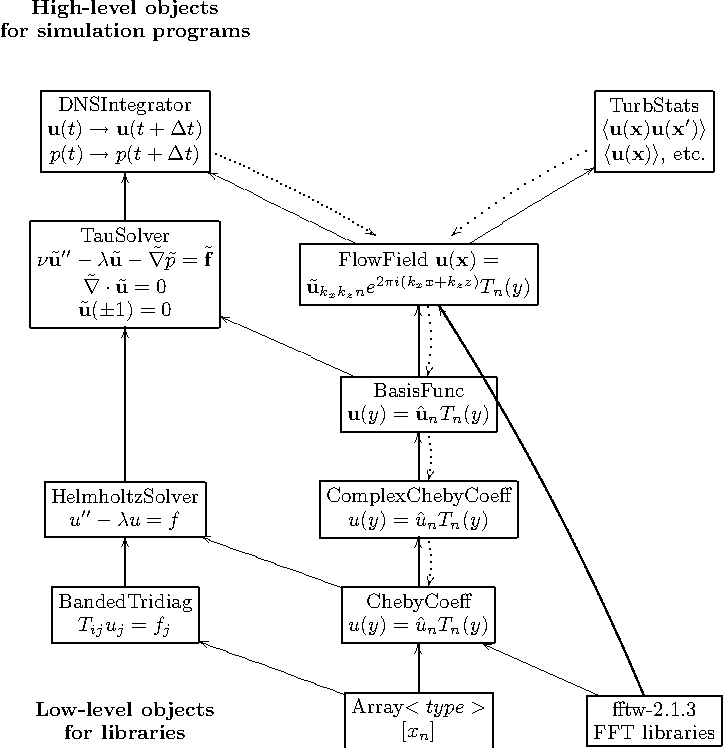
\includegraphics[width=6.0in]{cfstructure}
\end{center}
\caption{{\bf Structure of Channelflow software.}}
\label{fig:cfstructure}
\end{figure}


\subsection{Extending Channelflow}
\label{sec:extensions}
To be written.

\section{Validation}

\subsection{Integration of Orr-Sommerfeld eigenfunctions}

\subsection{Law of the wall in a channel flow}

Figure \ref{fig:walllaw} compares the mean velocity profile of a turbulent
channel flow computed with Channelflow to theoretical and experimental
scaling laws. The figure is plotted in ``wall units''. Define the
{\em friction velocity} $u_*$ by
\begin{align}
u^* \defn \sqrt{\nu \frac{dU}{dy} \bigg|_{y=0}}
\end{align}
where $U(y)$ is the mean velocity profile. The wall-units for lengths
and velocities are then defined by
\begin{align}
y_+ &\defn y u^*/ \nu \\
U_+ &\defn U/u^*
\end{align}
In these units the mean flow of a turbulent channel flow obeys
\begin{align}
U_+ &= y_+  \qquad \quad \qquad \text { in the viscous sublayer } y_+ < 10 \\
U_+ &= 2.5 \ln y_+ + 5 \;\;\; \text { in the inertial layer } \quad \; \; y_+ > 30
\end{align}
For a derivation of the scaling laws, see Tennekes and Lumley
(\cite{Tennekes72}) Section 5.2. The mean velocity profile shown in
Figure \ref{fig:walllaw} was computed by {\tt walllaw.cpp} in the {\tt
examples/source} directory. The computation uses a $48 \times 97
\times 24$ grid on a domain of size $(L_x, L_y, L_z) =
(4\pi/3,2,2\pi/3)$, with viscosity $\nu = 1/4000$, resulting in a
centerline-velocity Reynolds number of $\Rey = 3110$ and $u^* = 0.0450$.
Integration was RK3 with rotational nonlinearity calculation and
dealiasing in $xz$, with constant mass flux enforced.

\begin{figure}
\centering
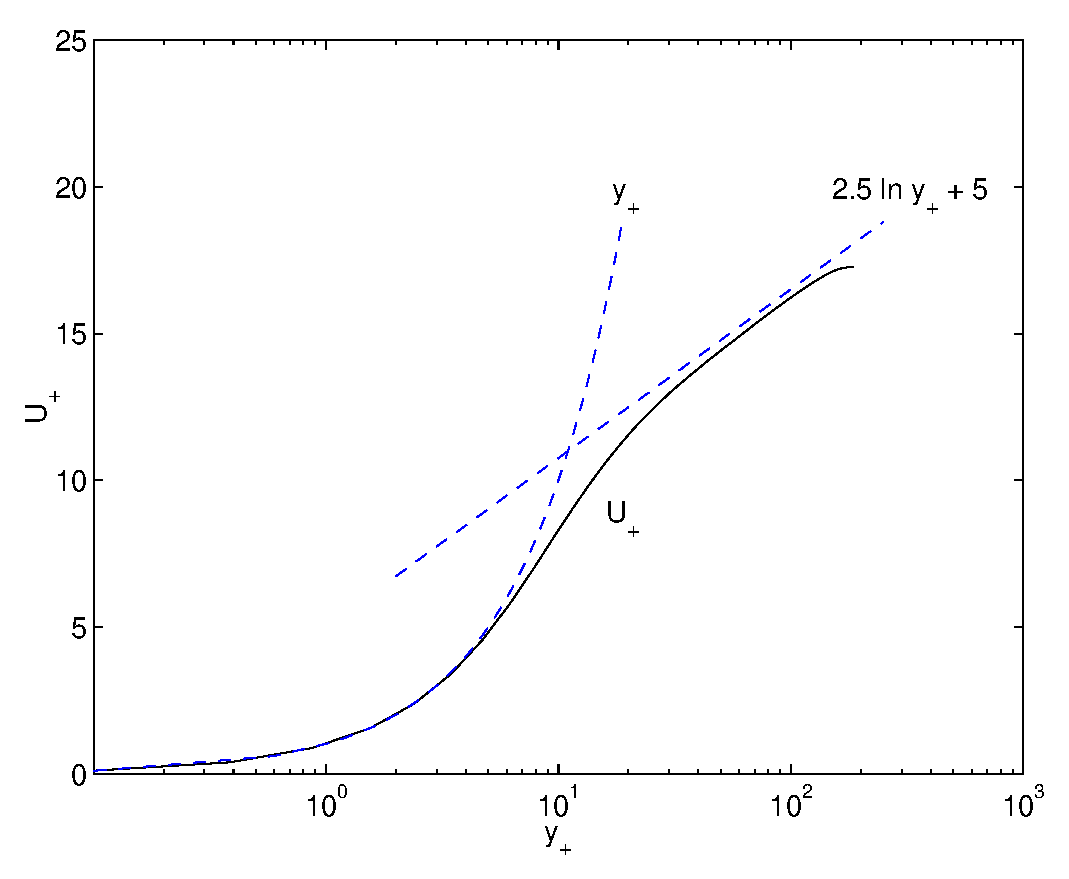
\includegraphics[height=3.0in]{walllaw}
\caption{{\bf The law of the wall.} Mean velocity of a turbulent channelflow
compared to scaling laws for the viscous sublayer ($U/u^* \approx y_+$) and
the inertial layer ($U/u^* \approx 2.5 \ln y_+ + 5$).}
\label{fig:walllaw}
\end{figure}



\section{Benchmarks}

\subsection{Speed}
\label{sec:speed_benchmarks}

Channelflow owes its speed to Matteo Frigo and Steven G.\ Johnson's
powerful and elegant FFTW, the Fastest Fourier Transform in the West
(\cite{Frigo98}). Comparisons to Fortran to be redone and written.

\subsection{Memory}
\label{sec:memory_benchmarks}

There is some memory overhead associated with programming in C++.
First, C++ programming style encourages use of class member data
in order to make objects as independent and self-contained as possible.
Second, C++ compilers introduce extra data fields into objects for
things like virtual function pointers. These effects can compound
quickly when objects contain other objects, or worse, arrays of other
objects.

My policy in writing Channelflow was to pay close attention to these
effects on large or heavily used objects, where there might be significant
cost, but to incur small memory overhead when it resulted in better
modularization. The FlowField class, for example, has a array of
Reals of length $dN^3$ for storing $d$-dimensional real-valued data on
an $N \times N \times N$ grid. (For simplicity, let $N_x = N_y = N_z$ in
this section.) But FlowField also has several small constant-length data
members, which facilitate independence between multiple FlowField objects,
and a few $N$-length arrays, which cache precomputed trigonometric
functions. As as result, the size of a FlowField is roughly
$d N^3 + a N + b$ reals, where $a$ and $b$ are $O(10)$. For typical
$N$, the $a N + b$ overhead is negligible. Lastly, Channelflow makes
minimal use of inheritance and virtual functions, because in my
experience, those features make C++ code hard to understand.

To check that C++ memory overhead was in fact negligible, I compared
the actual memory consumption of running programs to scaling-law
estimates. The scaling laws are derived from the formula
\begin{align}
\text{\# megabytes} = (\text{\# scalar fields}) \times \frac{N^3 \text{ Reals}}{\text{scalar field}} \times
\frac{8 \text{ bytes}}{\text{Real}} \times \frac{1 \text{ megabyte}}{2^{20} \text{bytes}}
\end{align}
The minimal set of data for second-order time-stepping has 14 scalar
fields, from the four three-dimensional fields $\bu^{n+1}, \bu^n, \bff^n,
\bff^{n-1}$, and the two scalar fields $q^{n+1}$ and $q^n$, giving a
minimal estimate of $14 \times 2^{-17} N^3$ MB.\footnote{Clever use of
memory during timestepping calculations could probably reduce the number of
fields stored below fourteen, but memory is cheap enough that the savings
isn't worth the cost to intelligibility of the code.} The CNAB TauSolver
caches 6 additional precomputed scalar fields $q_0, v_0, q_+, v_+,
q_-, v_-$ for influence-matrix calculations (as noted in Section
\ref{sec:influence_matrix}), resulting in an CNAB estimate of $20
\times 2^{-17} N^3$. The RK3 TauSolver caches these 6 additional
precomputed scalar fields for each of 3 Runge-Kutta substeps,
resulting in an RK3 estimate of $32 \times 2^{-17} N^3$ MB.

\begin{figure}
\centering
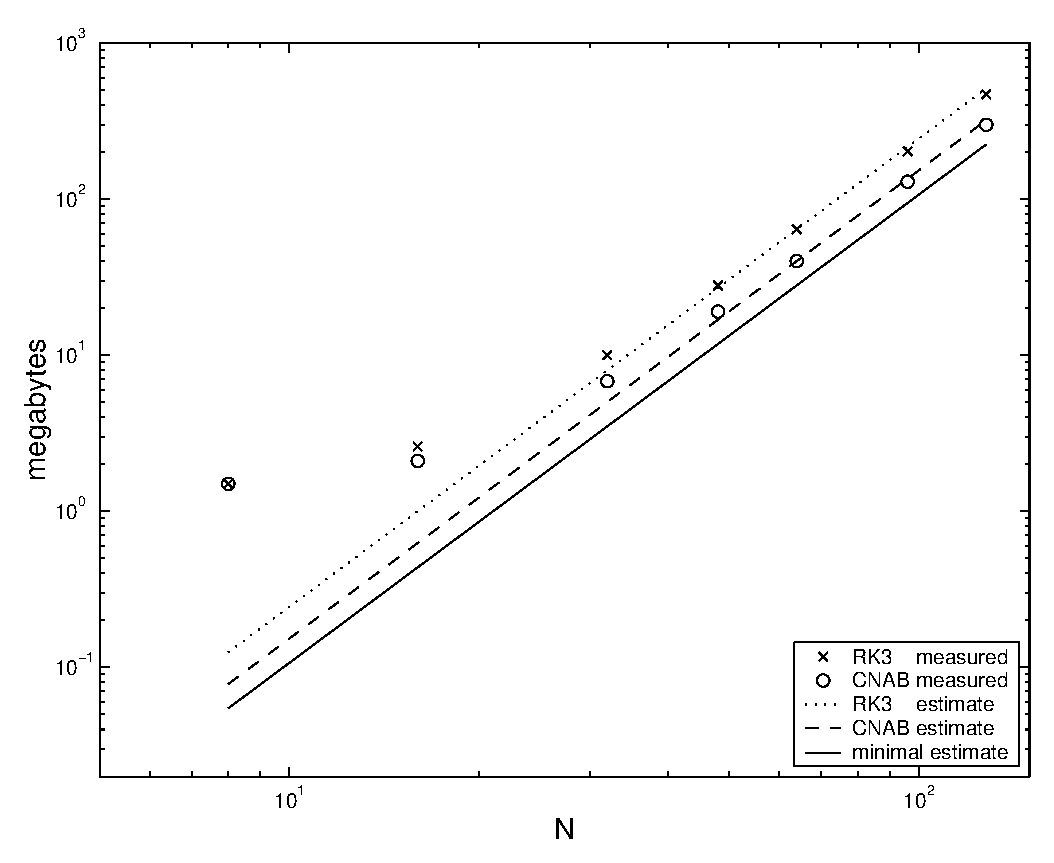
\includegraphics[height=3.0in]{memory}
\caption{{\bf Memory consumption as function of gridsize.} Comparison of
actual memory consumption to scaling-law estimates.}
\label{fig:memory}
\end{figure}

Figure \ref{fig:memory} compares the actual memory consumption
measured by the GNU ``top'' utility to the scaling-law estimates. The
memory overhead is small for $N=32$ and negligible beyond that. Note
that the overhead includes the $C$ libraries, I/O facilities, etc.,
which accounts for the departure from estimates for small
$N$.\footnote{For the truly pedantic, note that the estimates for CNAB
and RK3 very slightly {\em overestimate} memory consumption for large
$N$. This is due to the lack of caching of precomputed $(q, v)$ fields
for aliased Fourier modes.} Note also, from the scaling-law formula
and the figure, that the memory overhead for caching precomputed $(q,
v)$ fields for the influence-matrix method is roughly a factor of
$3/2$ for CNAB and $2$ for RK3. Future releases will probably have an
option to eliminate caching at the cost of speed.

\section{Software issues}
\label{software}

\subsection{Installation}
\label{sec:installation}

\subsection{Debugging}
\label{sec:debugging}

The Channelflow library code contains hundreds of safety checks on things
like array bounds and Physical/Spectral states of ChebyCoeff and FlowFields.
These safety checks are turned off in the optimized libraries. If your
Channelflow program produces a segmentation violation or bizarre numerical
results, you should recompile your code with debugging flags on and relink
to the debugging libraries. For example, for the program foo.cpp,
run ``make foo.dx'' and then either run foo.dx on the console or in a
debugger such as gdb. I often set ``break exit'' in gdb so that I can
examine the stack at the moment of exit. For more information on debugging,
consult the gdb manual.

\bibliographystyle{plain}
\bibliography{channelflow}


\end{document}
